\chapter{Background and Related Work}
\label{chp:related_work}

\epigraph{The study is to proceed on the basis of the conjecture that every aspect of learning or any other feature of intelligence can in principle be so precisely described that a machine can be made to simulate it. \textnormal{[...]} We think that a significant advance can be made in one or more of these problems if a carefully selected group of scientists work on it together for a summer.}{McCarthy et al., 1955, Proposal for the Dartmouth conference}

The primary goal of this thesis is to implement an associative memory model as a spiking neural network on top of neuromorphic hardware. In this chapter we aim at providing a terse summary of the mentioned fields: \cref{sec:neural_network_models,sec:biophysical_neuron_model,sec:spiking_neuron_models} address artificial neural network models in general, the neurobiological concepts inspiring spiking neural networks, relevant spiking neuron models, and their parameters. \cref{sec:neuromorphic_hardware} focuses on the neuromorphic hardware systems in the \HBP. In \cref{sec:willshaw_theory} we discuss the notion of associative memories and expand on the Willshaw associative memory model relied upon in this thesis.

%
% HISTORY OF ARTIFICIAL NEURAL NETWORK MODELS
%

\section{History of artificial neural network models}
\label{sec:neural_network_models}

In 1780 Luigi Galvani discovered that the injection of electric potentials into animal muscle tissue causes contractions. He was the first to notice that electricity could play a role in the animation -- or liveness -- of animals and laid the groundwork for research concerning electrophysiology \cite{piccolino1997luigi}.

Sixty-eight years later, in 1848, Emil du Bois-Reymond discovered discrete electrical pulses generated by nerve cells \cite{pearce2001emil}. It took another seventeen years until Julius Bernstein (supported by du Bois-Reymond) could successfully record one of these \emph{action potentials} or \emph{spikes} on paper. Today we know that action potentials are the primary way of encoding information in the nervous system \cite{schuetze1983discovery}.

\begin{figure}
	\small
	\centering
	\subbottom[Pyramid cells]{
		\centering
		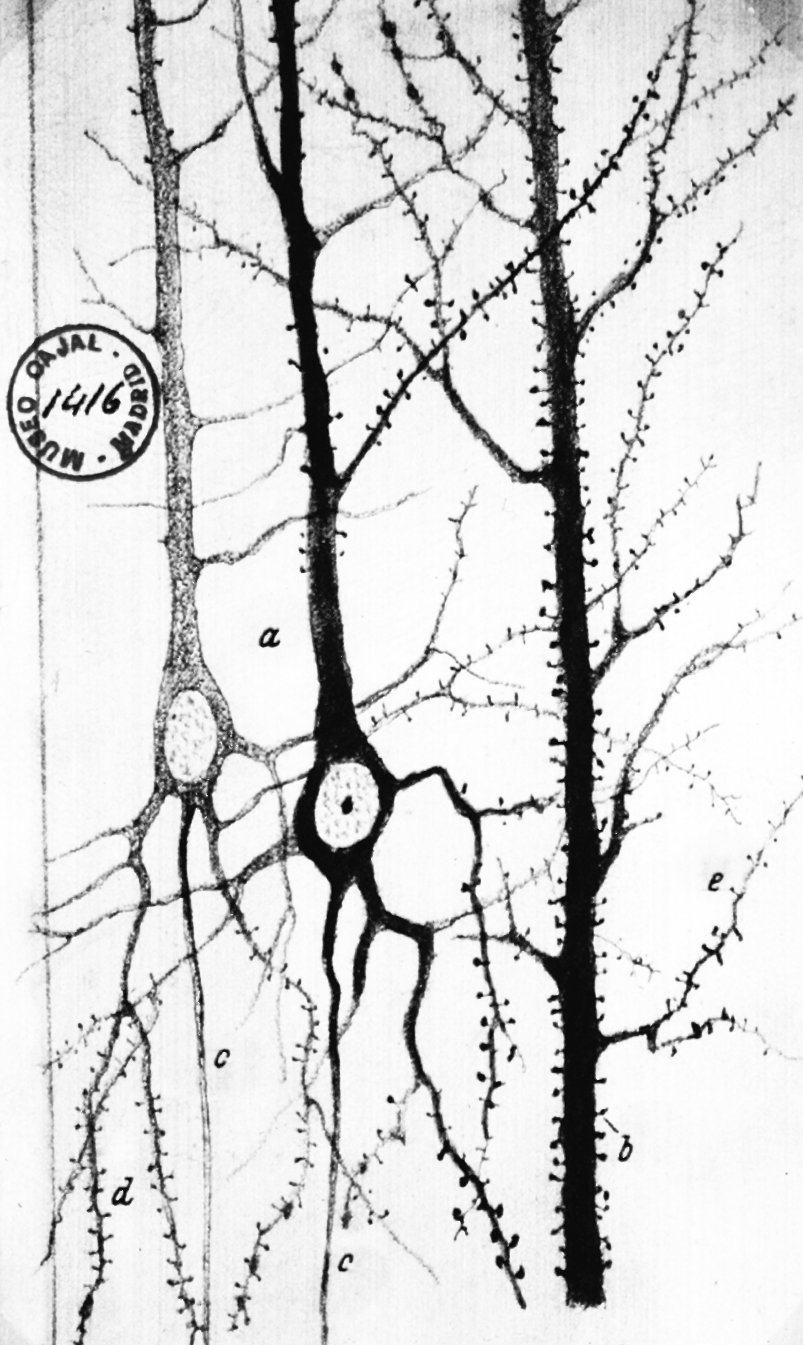
\includegraphics[height=7cm]{media/chp2/cajal_pyramid_cell.png}
		\label{fig:cajal_pyramid_cell}
	}
	\hspace*{0.75cm}
	\subbottom[Neurons in spinal marrow]{
		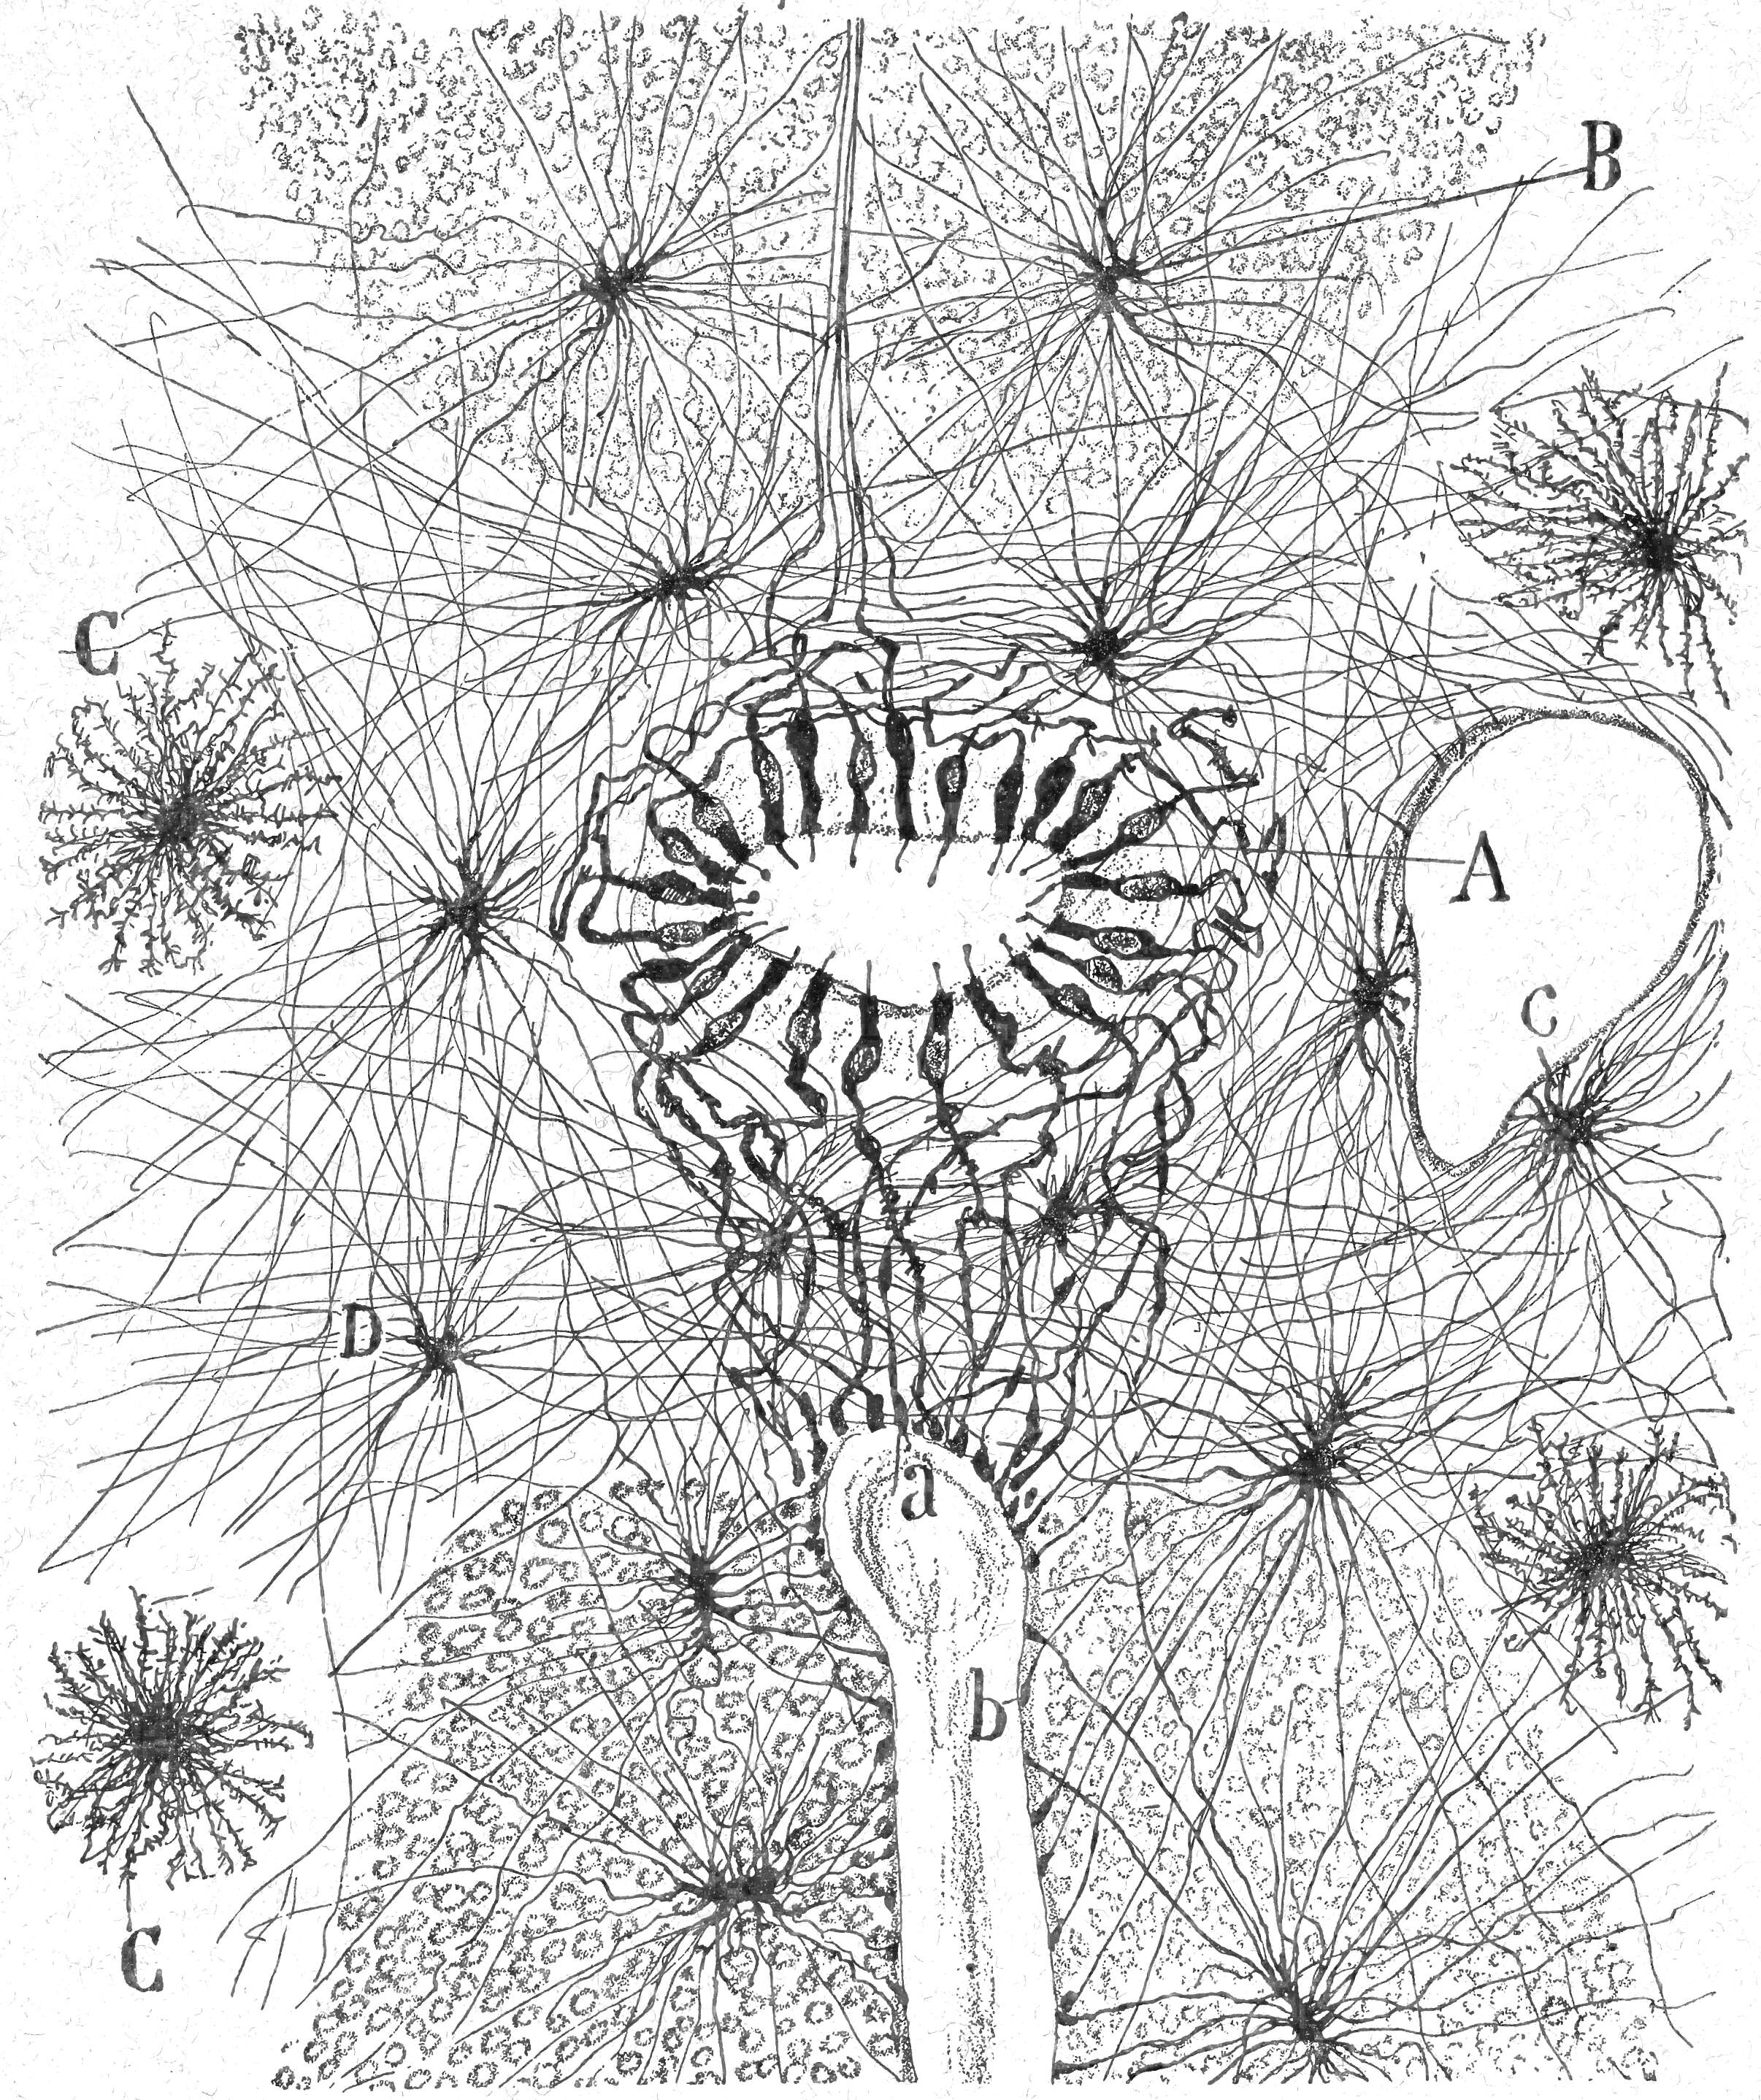
\includegraphics[height=7cm]{media/chp2/cajal_neuroglia.jpg}
		\label{fig:neurons_shape}
	}
	\caption[Drawings by Santiago Ramón y Cajal]{Neural tissue prepared using Golgis method and drawn by Santiago Ramón y Cajal around 1900. (a) shows pyramidal neurons in brain tissue, (b) neurons of varying shape in the white spinal marrow substance \cite{ramon1904textura}.}
	\label{fig:cajal}
\end{figure}
At the end of the nineteenth century, technological advances in microscopy and a new staining method invented by Camillo Golgi allowed scientists to examine individual neurons in brain and spinal tissue samples (\cref{fig:cajal}). In 1887 Santiago Ramón y Cajal was the first to propose neurons as distinct base units of information processing in biological systems. For their work Golgi and Cajal received the 1906 Nobel prize. Their discoveries gave rise to the \emph{neuron doctrine}, the idea that spinal cord and brain are made of basic building blocks -- neurons -- and their support structures \cite{glickstein2006golgi}.

As the understanding of the neurobiological mechanisms advanced, another question began to dawn in the scientific world: if animal -- and human -- behaviour was solely determined by the electrophysiological properties of neural networks, could it not be possible to build machines that simulate processes in the brain up to cognition and intelligence? In the 1940s researchers began to construct mathematical models which mimic structural properties of biological neural networks. The development of artificial neural networks since then can be broken down into three distinct generations \cite{maass1997networks}.

\subsection{First generation: binary McCulloch-Pitts cells}
\label{sec:mcculloch_pitts_neuron}

\marginfig{Sketch of a McCulloch-Pitts artificial neuron}{
	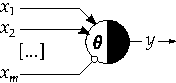
\includegraphics{media/chp2/mcculloch_pitts_neuron.pdf}
	\vspace{0.25cm}
}{Sketch of a McCulloch-Pitts neuron: excitatory (arrow) and inhibitory (circle) inputs are accumulated. If a threshold $\theta$ is passed, the output $y$ is set to one, zero otherwise.}{\label{fig:mcculloch_pitts_neuron}}
In 1943 Warren McCulloch and Walter Pitts proposed the first artificial neural network model. In order to cope with the high diversity and complexity of biological neurons, their model is based on several simplifying assumptions: the nervous system is built of a network of neurons, each consisting of a cell body (\emph{soma}) and an axon. They gather input from connected neurons through excitatory or inhibitory synapses located at dendritic extensions of the soma (\emph{dendrites}). If the excitation of a neuron passes a threshold, the neuron responds with a binary \enquote{all-or-none} spike, that travels along the axon to other neurons, where it is received as input (\cref{sec:biophysical_neuron_model,fig:neuron_sketch}).
\begin{figure}
	\centering
	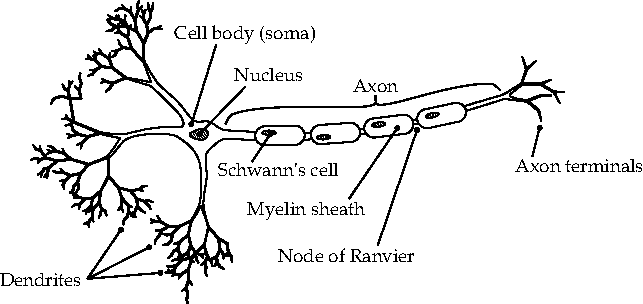
\includegraphics[width=\textwidth]{media/chp2/neuron_sketch.pdf}
	\caption[Sketch of a schematised model neuron]{Sketch of a schematised biological model neuron. Input spikes arrive at synapses located at the dendrites and are processed in the cell body. Resulting output spikes travel along the axon to the axon terminals, which connect to other neurons or a neuromuscular junction. Inspired by \cite{kandel2012principles}.}
	\label{fig:neuron_sketch}
\end{figure}
Furthermore, McCulloch and Pitts argue that transmission of signals along the axon is almost instantaneous and considerable delay occurs only at the synapses. This allows to disregard spike times and instead synchronously propagate binary values between neurons in discrete time steps \cite{mcculloch1943logical}.

\marginfig{McCulloch-Pitts artificial neuron as Boolean operators}{
	OR ($y = x_1 \vee x_2$):\\
	\vspace{0.25cm}
	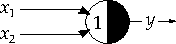
\includegraphics{media/chp2/mcculloch_pitts_neuron_or.pdf}
	\vspace{0.5cm}\\
	AND ($y = x_1 \wedge x_2$):\\
	\vspace{0.25cm}
	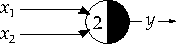
\includegraphics{media/chp2/mcculloch_pitts_neuron_and.pdf}
	\vspace{0.5cm}\\
	NOT ($y = \neg x$):\\
	\vspace{0.25cm}
	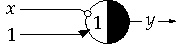
\includegraphics{media/chp2/mcculloch_pitts_neuron_not.pdf}
	\vspace{0.25cm}
}{McCulloch-Pitts artificial neuron as Boolean operators.}{\label{fig:mcculloch_pitts_neuron_logic}}
Mathematically, a single McCulloch-Pitts cell with binary input vector $\vec x = \transpose{(x_1, \ldots, x_m)} \in \B^m$, output $y \in \B$, and $\B = \{0, 1\}$ can be described as follows (\cref{fig:mcculloch_pitts_neuron})
\begin{align}
	y &= \Heaviside(\transpose{\vec w} \cdot \vec x - \theta) & \text{where} \quad 
		\Heaviside(x) &=  \begin{cases}
			1 & \text{if } x \geq 0 \\
			0 & \text{otherwise}
	    \end{cases} \,.
	\label{eqn:mcculloch_pitts_cell}
\end{align}
The weights $\vec w = \transpose{(w_1, \ldots, w_m)} \in \{-1, 1\}^m$ model excitatory ($w_i = 1$) or inhibitory ($w_i = -1$) synaptic connections to the input $x_i$, the threshold $\theta \in \mathbb{Z}$ describes the minimum excitation that causes a \enquote{one} as output. The function $\Heaviside(x)$ is also called \enquote{Heaviside step function}.

As shown in \cref{fig:mcculloch_pitts_neuron_logic}, the cells can be used to construct the basic operators of Boolean algebra. It follows that any computable function can be described by a large network of McCulloch-Pitts cells -- they are Turing complete \cite{copeland1996alan}.

\subsection{Second generation: firing-rate coded neural networks}

In 1958 Frank Rosenblatt extended the binary McCulloch-Pitts cell to the so called \enquote{perceptron}. Weights $w_i$ and neural input $x_i$ in \cref{eqn:mcculloch_pitts_cell} are now real-valued instead of binary. Biologically, this change can be motivated by the observation that some neurons operate in a mode known as \enquote{tonic spiking} in which they output discrete spikes at a certain rate that monotonously depends on the excitation of the neuron (Figures \ref{fig:neuron_behaviours}(a) and \ref{fig:neuron_behaviours}(g)). The real valued input $\vec x \in \R^m$ can be interpreted as the average firing-rate of the pre-synaptic neuron, the weights $\vec w \in \R^m$ describe the influence of a synapse on the excitation of the neuron \cite{haykin2011neural}.

Rosenblatt's most important contribution, though, is a learning rule which allows to train the weights $\vec w$ in such a way, that the perceptron outputs a desired answer $y_k$ for a certain input $\vec x_k$, allowing to solve linear classification and regression tasks \cite{minsky1987perceptrons}.

\marginfig{Sketch of a classical artificial neuron}{
    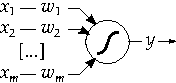
\includegraphics{media/chp2/classical_neuron.pdf}
    \vspace{0.25cm}
}{Sketch of a firing-rate coded artificial neuron. Each neuron in the network computes the weighted sum of inputs $x_1, \ldots, x_m$, applies a non-linearity $f$ and outputs an activation value $y$ that might be fed into other neurons or act as part of the network output.}{\label{fig:classical_neuron}}
In the context of the feed-forward \MLP, the neuron model is generalised to the \enquote{firing-rate artificial neuron}, replacing the Heaviside function $\Heaviside$ with an arbitrary non-linear, sigmoid function $f$ and fusing the threshold $\theta$ as an additional dimension (\enquote{bias}) into the input $\vec x$ and the weights $\vec w$ (\cref{fig:classical_neuron})
\begin{align}
	y = f(\transpose{\vec w} \cdot \vec x) \,.
\end{align}
The weights $\vec w$ of the individual neurons in a \MLP can be easily trained using the back-propagation algorithm (a generalisation of Rosenblatt's perceptron learning rule). Today, with the broad availability of massively parallel computing hardware, large {\MLP}s with many hidden layers are employed with success in the field of \enquote{deep learning} \cite{hinton2006fast}.

\subsection{Third generation: spiking neural networks}

McCulloch and Pitts assumed that coarse, discrete timesteps are sufficient for the propagation of neural output -- a paradigm that is adopted by second generation networks. Experiments suggest however, that exact spike timing and spike time correlation within neuron populations are used to encode information in the nervous system \cite{shadlen1994noise}. At the end of the 1980s, these discoveries gave rise to the third generation of neural networks, in which neurons are simulated as dynamical systems with asynchronously generated binary spikes \cite{maass1997networks}.

Besides being closer to biology, spiking neural networks have several practical advantages over their predecessors: whereas firing-rate models require the transfer of the neuron state of every neuron in every time step, the asynchronicity of spiking networks only requires communication whenever a neuron generates a spike. Due to the loose coupling of individual neurons, spiking networks lend themselves to be simulated energy efficiently on massively parallel, asynchronous hardware. Furthermore, given their time-dynamic nature, spiking neural networks intrinsically process time series of data.

On the other hand, simulation of neuron time dynamics is computationally intensive, training of spiking networks is more complicated compared to their firing-rate counterpart and -- at least for simple models -- biological plausibility is still limited: usually neither spatiality, nor the influence of neuromodulators are simulated. Nevertheless, spiking neural networks may provide a useful simulation platform for entire brain circuits \cite{johansson2007towards} and may in the future allow to simulate deep networks on specialised, energy efficient hardware \cite{hasler2013finding,schmidhuber2015deep}.

We continue with a description of the spiking neural network models this thesis is based on in \cref{sec:spiking_neuron_models}, but before, in \cref{sec:biophysical_neuron_model}, we quickly explore their biological basis.

%
% BIOPHYSICAL NEURON MODEL
%

\section{Biophysical neuron model}
\label{sec:biophysical_neuron_model}

Biological observations of neuronal behaviour have (amongst others) been captured in the biophysically meaningful \HH neuron model, introduced in 1952  \cite{hodgkin1952quantitative}. It builds the basis of most simplified spiking neural network models in neuroinformatics. In the remainder of this section we discuss the relevant parts of this model.

\subsection{Passive electrophysiological properties of the neuron membrane}
\label{sec:electrophysiological_properties}

\marginnote{Ions in the intra-/extra\-cel\-lu\-lar fluid which usually play a role in neurobiological processes are: sodium ions \(\mathrm{Na}^+\), chloride \(\mathrm{Cl}^-\), potassium ions \(\mathrm{K}^+\), calcium ions \(\mathrm{Ca}^{2+}\), as well as negatively charged amino acids \(\mathrm{A}^-\).}
The electrical properties of a single neuron are caused by a different ion compositions in intra- and extracellular fluid, and selectively permeable ion channels in the cell membrane. When measuring the electrical potential between the intra- and extracellular space -- the \emph{membrane potential} {\um} -- of an inactive neuron, one finds the intracellular space being more negatively charged than the extracellular space \cite{kandel2012principles}. This particular voltage is called the \emph{resting} or \emph{leak} potential \El.

\begin{figure}
	\centering
	\subbottom[Membrane without \(\mathrm{K}^+\)-channel]{%
		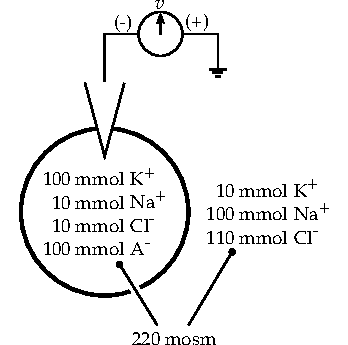
\includegraphics{media/chp2/neuron_channel_a.pdf}%
		\label{fig:neuron_channel_a}
	}%
	\subbottom[Added \(\mathrm{K}^+\)-channel]{%
		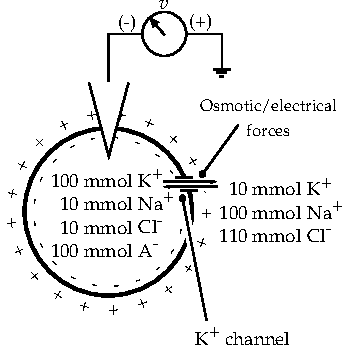
\includegraphics{media/chp2/neuron_channel_b.pdf}%
		\label{fig:neuron_channel_b}
	}
	\caption[Membrane potential change caused by selectively permeable ion channel]{Ion compositions in intra- and extracellular space and with closed (a) and opened (b) selectively permeable ion channel. See \cref{sec:electrophysiological_properties} for a description. Adapted from \cite{kandel2012principles}.}
\end{figure}
An examination yields differences in the intra- and extracellular fluid ion-composition, with the intracellular composition being maintained by ion pumps in the cell membrane. However, seemingly contradictory to the previous result, both fluids are electrically neutral and have the same osmotic concentration. Only if the membrane was a perfect insulator -- as assumed in \cref{fig:neuron_channel_a} --, there would be no measurable potential.

\marginnote{The number of ions involved in the generation of the equilibrium potential is negligibly small compared to the total number of ions in the cell.}
Experiments show, that the membrane contains selectively permeable ion channels. In its resting state, the membrane is mostly permeable for potassium ions $\mathrm{K}^+$. Due to the difference between intra- and extracellular ion concentration, an osmotic force causes \(\mathrm{K}^+\) to flow out of the cell. The total ionic current is proportional to the number channels in the membrane, or its \emph{permeability} for \(\mathrm{K}^+\). Missing \(\mathrm{K}^+\) cause the intracellular fluid to become slightly negatively charged, creating a countering electric force on the positively charged ions. As sketched in \cref{fig:neuron_channel_b}, the system converges towards an equilibrium state with potential $E_{\mathrm{Eq}}$ in which osmotic and electric force are equal.

Consider the equilibrium potential $E_{\ion}$ for a membrane that is permeable for an ion species \ion only. We refer to $E_{\ion}$ as the \emph{reversal potential} for \ion: its ionic current reverses at this potential. For intra- and extracellular ion concentrations $[\ion]_{\mathrm{in}}$ and $[\ion]_{\mathrm{out}}$, $E_{\ion}$ is given according to the Nernst equation as
\begin{align}
	E_{\ion} &= \frac{R \cdot T}{z \cdot F} \cdot \ln\left( \frac{[\ion]_{\mathrm{out}}}{[\ion]_{\mathrm{in}}} \right){,}
	\label{eqn:nernst}
\end{align}
where $R$ is the ideal gas constant, $T$ the temperature in Kelvin, $F$ Faraday's constant, and $z$ the ion charge in elementary charges \cite{kandel2012principles}.
Given the (relative) permeabilities or \emph{conductances} $g_{\ion}$ of the cell membrane for each ion species \ion, the equilibrium potential $E_{\mathrm{eq}}$ can be calculated according to the Goldman–Hodgkin–Katz equation as
\begin{align}
	E_{\mathrm{eq}} = \frac{\sum\nolimits_{\ion} g_{\ion} \cdot E_{\ion}}{\sum\nolimits_{\ion} g_{\ion}} = \frac{\sum\nolimits_{\ion} g_{\ion} \cdot E_{\ion}}{g_{\mathrm{tot}}} \,.
	\label{eqn:membrane_base}
\end{align}
\marginnote{Correspondence between Fig.~\ref{fig:membrane_base} and Eq.~(\ref{eqn:membrane_base}) can be easily shown using Kirchhoff's laws.}
The behaviour modelled by \cref{eqn:membrane_base} corresponds to an electric circuit, consisting of parallel voltage sources with voltage $E_{\ion}$ and a series resistor with conductance $g_{\ion}$ for each ion channel (\cref{fig:membrane_base}).

\begin{figure}
	\small
	\centering
	\begin{circuitikz}
		\draw[->] (-1.5, 0.5) -- node[left] {\Eeq} (-1.5, 3.5);
		\draw(0, 4) to[R, l=$g_{\mathrm{K}^+}$] (0, 2);
		\draw(0, 2) to[battery1, l=$E_{\mathrm{K}^+}$] (0, 0);
		\draw(2, 4) to[R, l=$g_{\mathrm{Na}^+}$] (2, 2);
		\draw(2, 0) to[battery1, l=$E_{\mathrm{Na}^+}$, mirror] (2, 2);
		\draw(4, 4) to[R, l=$g_{\mathrm{Cl}^-}$] (4, 2);
		\draw(4, 2) to[battery1, l=$E_{\mathrm{Cl}^-}$] (4, 0);
		\draw(-1.5, 0) to[short, o-*]
		     (0, 0) to[short,-*]
		     (2, 0) to[short,-*] (4, 0);
		\draw(-1.5, 4) to[short, o-*]
		     (0, 4) to[short,-*]
		     (2, 4) to[short,-*] (4, 4);
		\draw[dashed] (4, 0) -- (6, 0) -- (6, 1.85);
		\draw[dashed] (6, 2.15) -- (6, 4) -- (4, 4);
		\draw (6, 1.85) to[C, l=$\Cm$] (6, 2.15);
		\draw[->,dashed] (7, 0.5) -- node[right] {$\um(t)$} (7, 3.5);
	\end{circuitikz}
	\caption[Model equivalent circuit diagram of the neuron membrane for three ion channels]{Model equivalent circuit diagram of the neuron membrane for three ion channels. The potential that can be measured across the terminals on the left (without the capacitor) corresponds to the equilibrium potential as described in equation \cref{eqn:membrane_base}. Introducing a capacitor (dashed) with capacitance $\Cm$ transforms the circuit into the time-dynamic neuron base model in \cref{eqn:membrane_base_time}.}
	\label{fig:membrane_base}
\end{figure}
Due to inertia in the system, the membrane potential adapts slowly to any change, for example changes in the ion channel permeabilities. As depicted in \cref{fig:membrane_base}, this time-dynamic can be modelled by adding a capacitor with capacitance {\Cm} -- the \emph{membrane capacitance} -- in parallel to the equivalent circuit.

\begin{figure}
	\centering
	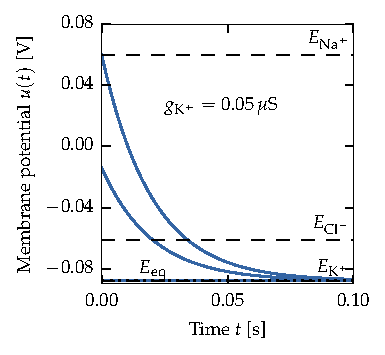
\includegraphics[trim=0.1cm 0.75cm 0.25cm 0.1cm,clip]{media/chp2/base_membrane_eq1.pdf}
	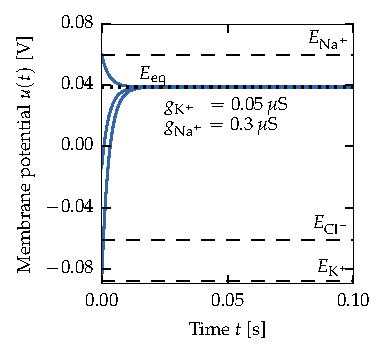
\includegraphics[trim=0.75cm 0.75cm 0.25cm 0.1cm,clip]{media/chp2/base_membrane_eq2.pdf}
	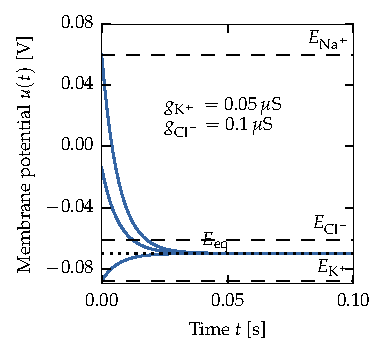
\includegraphics[trim=0.1cm 0.1cm 0.25cm 0.1cm,clip]{media/chp2/base_membrane_eq3.pdf}
	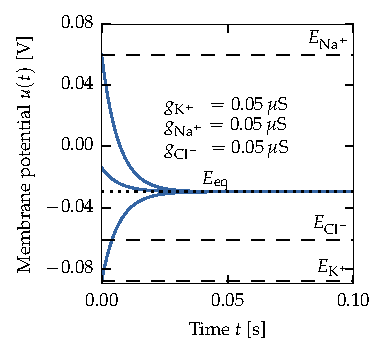
\includegraphics[trim=0.75cm 0.1cm 0.25cm 0.1cm,clip]{media/chp2/base_membrane_eq4.pdf}
	\caption[Membrane potential over time for varying membrane conductances]{Membrane potential over time for varying membrane conductances, according to \cref{eqn:membrane_base_time}. The reversal potentials are set to $E_{\mathrm{K}^+} = \SI{-88}{\milli\volt}$, $E_{\mathrm{Na}^+} = \SI{61}{\milli\volt}$ and $E_{\mathrm{Cl}^-} = -\SI{60}{\milli\volt}$, the membrane capacitance \Cm to $\SI{1}{\nano\farad}$.}
	\label{fig:membrane_base_time}
\end{figure}
\marginnote{By convention, positive currents $i(t)$ drive the membrane potential towards more negative values, negative currents towards more positive values.}
The time differential of the voltage across the capacitor \(\dum(t)\) is proportional to the current $i(t)$, which in turn is proportional to the difference \(\um(t) - \Eeq\). Hence, the circuit can be described as a linear differential equation
\begin{align}
	- \Cm \cdot \dot u(t) = i(t)
		&= g_{\mathrm{tot}} \cdot (u(t) - E_{\mathrm{eq}})
		 = \sum\nolimits_{\ion} g_{\ion} \cdot (u(t) - E_{\ion}) \,.
	\label{eqn:membrane_base_time}
\end{align}
\cref{fig:membrane_base_time} shows the system for varying $u_0$ and different membrane conductances. In all four plots the membrane is always slightly permeable for potassium ions \(\mathrm{K}^+\). If the membrane is not permeable for any other ion, this causes \(u(t)\) to slowly converge towards \(E_{\mathrm{K}^+}\). The velocity of the convergence is proportional to \(g_{\mathrm{tot}}\). Permeability for chloride or sodium ions pulls \(u(t)\) towards their reversal potential.

\subsection{Action potentials}

\begin{figure}
	\small
	\centering
	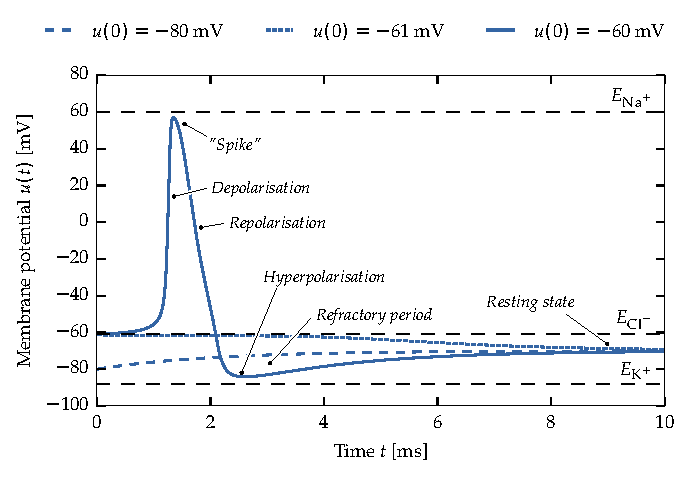
\includegraphics{media/chp2/hh_ap2_annotated.pdf}
	\caption[Annotated sketch of an action potential]{Annotated sketch of an action potential as produced by the \acrfull{HH} model. The membrane potential of three neurons is clamped to certain membrane potentials $\um(t)$ at $t = 0$. If a certain threshold potential is reached, the neuron generates an action potential; below this potential behaviour similar to a passive membrane can be observed.}
	\label{fig:action_potential_sketch}
\end{figure}

A passive cell membrane is not sufficient to explain action potentials and thus lacks an integral part of spiking neural networks -- the spikes. As soon as the neuron membrane potential surpasses a certain threshold $\ETh$, the neuron will suddenly depolarise up to a value $E_{\mathrm{spike}}$, followed by a decrease below the resting potential $\El$ (hyperpolarisation) to the reset potential $\Ereset$. The neuron stays close to the reset potential for a certain time span (known as \enquote{refractory period}), until the membrane potential again converges towards $\El$ (\cref{fig:action_potential_sketch}).

\marginnote{Ion channels are binary: they can either be open or closed -- the \HH model therefore describes the ion channel state probabilistically over a population of channels as three state variables in addition to the membrane potential.}
Mechanistically, this behaviour is produced by voltage-gated sodium and potassium ion channels ($\mathrm{Na^+}$, $\mathrm{K^+}$): the probability of open $\mathrm{Na^+}$ channels increases with the membrane potential, causing a positive feedback loop and a depolarisation of the membrane up to \Espike. Meanwhile, the voltage-gated channels for $\mathrm{K}^+$ open with the same mechanism, albeit a little slower, and the $\mathrm{Na}^+$ channels transition into a closed and deactivated state, causing the sudden re- and hyperpolarisation. Facilitated by the hyperpolarisation the $\mathrm{Na}^+$ and $\mathrm{K}^+$ channels reset to their initial state, allowing the generation of new action potentials \cite{kandel2012principles}.

An evolutionary (ultimate) explanation of action potentials is their suitability for signal propagation along the axon. As the neuron membrane is neither a perfect insulator nor the intracellular fluid a good conductor, pure electric signals are dampened with increasing spatial distance.
\marginnote{Spiking signals in biology can be explained with similar rationale as digital representations in computers: discrete signals can recover from noise without information loss, whereas analogue signals are irrecoverably altered.}
\enquote{All-or-none} spikes on the other hand allow constant signal renewal without information loss: as depicted in \cref{fig:neuron_sketch}, portions of the axon are insulated with \emph{Myelin} (decreasing the leak-conductance and thus the potential gradient), allowing fast but lossy electrical propagation of the signal. The Myelin sheath is regularly interrupted by \emph{Nodes of Ranvier}, where the neuronal ion-channel action potential generation mechanism renews the action potential \cite{kandel2012principles}.

\subsection{Chemical synapses}
\label{sec:biological_synapses}

\begin{figure}
	\centering
	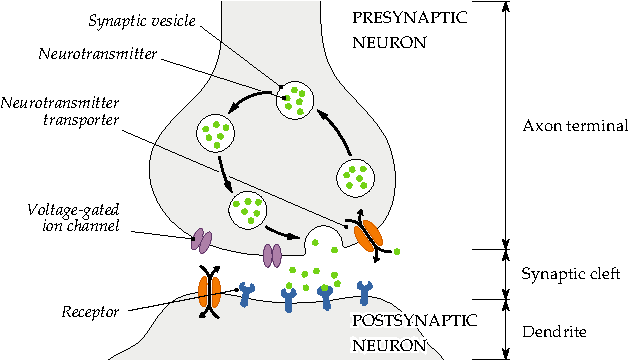
\includegraphics{media/chp2/SynapseSchematic_en.pdf}
	\caption[Chemical synapse schematic]{Chemical synapse, adapted from \url{https://commons.wikimedia.org/wiki/File:SynapseSchematic_en.svg}. See text for description.}
	\label{fig:chemical_synapse}
\end{figure}

As already mentioned in the discussion of artificial neural network models (\cref{sec:neural_network_models}), synapses are the basis for inter-neuron communication and thus neural networks. There are two types of biological synapses: electrical synapses, which allow for a direct exchange of intracellular fluid, and the more common chemical synapses, sketched in \cref{fig:chemical_synapse} and described in the following. If an action potential arrives at the axon terminal of the presynaptic neuron, vesicles containing a neurotransmitter fuse with the cell membrane and release the transmitter into the synaptic cleft. The transmitter then docks onto receptors located at the dendrites of the postsynaptic neuron, where they -- depending on the configuration of the dendritic part of the synapse -- trigger the opening or closing of ion channels and either excite or inhibit the neuron (pull the membrane towards more positive or negative potentials) \cite{kandel2012principles}.

% low-pass filters oder low-pass-filters
Compared to the spike transmission along the axon, the delay occurring at the synapse is rather large. The release of a neurotransmitter furthermore low-pass filters the incoming spikes, stretching their effect over longer time-periods.

\section{Simplified neuron and synapse models}
\label{sec:spiking_neuron_models}

\begin{figure}[t]
	\centering
	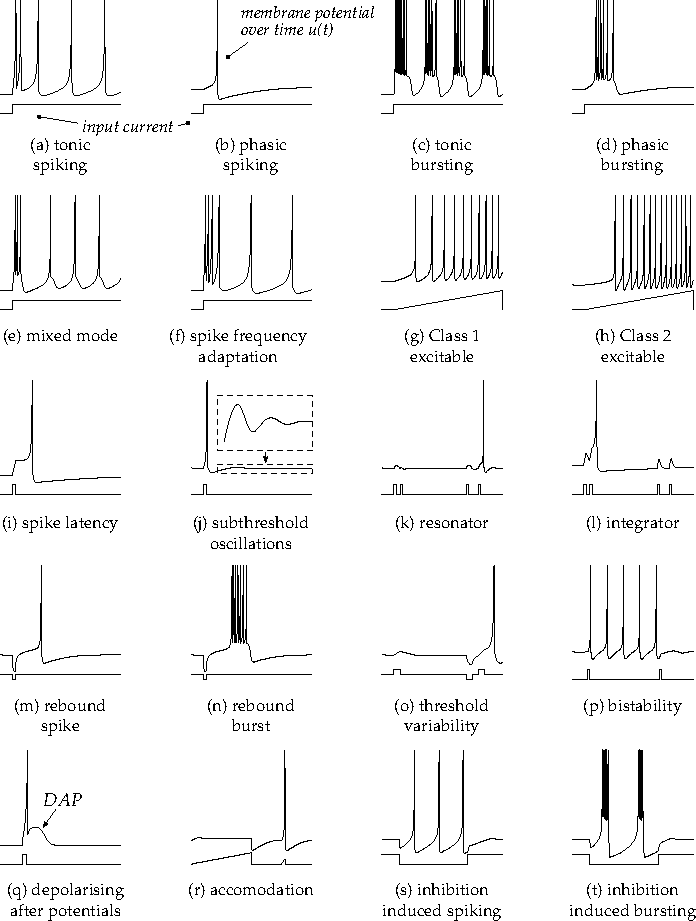
\includegraphics{media/chp2/izhikevich_whichmod_figure1.pdf}
	\caption[Sketches of spiking neuron behavioural patterns]{Sketches of spiking neuron behavioural patterns. Each subgraph shows membrane potential $\um(t)$ and input current $\isyn(t)$ over time. See \cite{izhikevich2004model} for more information. Electronic version of the figure and reproduction permissions are freely available at \url{http://www.izhikevich.com/}.}
	\label{fig:neuron_behaviours}
\end{figure}

The previous sections sketched two extremes: the biophysically meaningful \acrfull{HH} model, and the simplistic firing-rate neuron models used in machine learning. While it is surely possible to use the \HH model as the underlying neuron model for artificial spiking neural networks, its evaluation is computationally expensive \cite{izhikevich2004model} and mathematical analysis is complicated due to its intricate dynamics.

\marginnote{As discussed in \cite{izhikevich2004model}, the \HH model requires up to two magnitudes more floating point operations for the same time\-span as comparably expressive, but simpler models.}
To overcome these limitations, less complex neuron models have been developed. However, their reduced complexity often comes at the cost of reduced expressiveness: \cref{fig:neuron_behaviours} shows the variety of neuron behaviours observed in biological neurons that -- given the correct neuron parameters -- can be described with the \HH model. Yet, the simplest neuron models only support basic modes of operation (\eg \enquote{tonic spiking}). In the remainder of this section we introduce the synapse and neuron models used on the \acrshort{HBP} neuromorphic hardware platforms, list their parameters, and discuss their expressiveness. More information on spiking neuron models can be found in \cite{gerstner2002spiking}.

\subsection{Neuron model base equation}

\marginnote{A summary of the relevant neuron model parameters is given in \vref{tbl:adex_parameters}.}
The representation of the cell membrane as a capacitor with capacitance $\Cm$ is the conceptual basis of most spiking neuron models. Over time the capacitor is charged and discharged by two currents: the intrinsic channel current $\ichan(u, t)$, corresponding to the sum of ionic currents through the ion channels, and the synaptic -- or external -- current $\isyn(\um, t)$ modelling the ionic currents in the synapses as response to external input
\begin{align}
	- \Cm \cdot \dum(t) &= \im(t) = \ichan\left(\um(t), t\right) + \isyn\left(\um(t), t\right) \,.
	\label{eqn:simple_membrane_base_time}
\end{align}
The form of the channel current \ichan depends on the concrete neuron model, whereas the synaptic current \isyn is determined by the synapse model.

\subsection{Synapse models}
\label{sec:synapse_models}

\marginnote{The synapse model is usually independent of the neuron model -- synapses are solely a biologically inspired way to inject a current into a neuron. However, the boundaries will become fuzzy as we introduce excitatory and inhibitory synapses.}
Generally, the synaptic current \isyn is the sum of currents induced by all synapses of a neuron (the number of synapses equals the fan-in of the neuron in the network)
\begin{align}
	\isyn(u, t) &= \sum_{k} \isynk(u, t) \,.
	\label{eqn:synaptic_sum}
\end{align}
The current \isynk caused by each individual synapse $k$ is determined by the internal synapse state. This state is modified whenever the synapse receives a pre-synaptic spike and steadily converges to a resting value. The amplitude of the modification depends on the synapse weight $\wsyn_k$. The physical unit of $\wsyn_k$ depends on the synapse model. Two synapse models are common: \emph{current}-based and \emph{conductance}-based synapses.

\paragraph{Current based synapses with exponential decay}
Synapses of this type do not possess additional state variables -- their sole state is the current \isynk itself. This model is particularly interesting as \isynk does not depend on \um, which in some cases enables fully analytical solutions of the differential in \cref{eqn:simple_membrane_base_time}. Whenever an input spike is received at time $t$, the current is increased by $\wsyn_k$ (in ampere). The synaptic current then exponentially decays to zero over time with time constant $\tau_k$, modelling the low-pass behaviour mentioned in \cref{sec:biological_synapses}. A single current based synapse $k$ can be described as
\begin{align}
	\isynk(t) &\gets \isynk(t) + \wsyn_k \quad \text{on spike for $k$ at } t
	\label{eqn:current_based_sypase} \\
	- \mathrm{d}/\mathrm{d}t \; \tau_k \cdot \isynk(t) &= \isynk(t) \,.
	\label{eqn:current_based_sypase_decay}
\end{align}

\paragraph{Conductance based synapses with exponential decay}
This synapse model is biologically more plausible as it models the transmitter gated membrane channels in biological synapses to a certain extent. As it is available on all neuromorphic hardware platforms, it is the model of choice in this thesis. In contrast to the current based channel, each synapse has a conductance $g_k$ as internal state. An input spike at time $t$ increases the conductance by $\wsyn_k$ (in siemens). As with the current based model, the state variable decays with the synapse-specific time constant $\tau_k$.
\begin{align}
	g_k(t) &\gets g_k(t) + \wsyn_k \quad \text{on spike for $k$ at } t
	\label{eqn:conductance_based_sypase} \\
	- \mathrm{d}/\mathrm{d}t \; \tau_k \cdot g_k(t) &= g_k(t)
	\label{eqn:conductance_based_sypase_decay}
\end{align}
The actual synaptic current \isynk depends on the state $g_k$, the current membrane potential \um and the synaptic channel reversal potential $E_k$.
\begin{align}
	\isynk(\um, t) &= g_k(t) \cdot (\um - E_k)
	\label{eqn:conductance_based_current}
\end{align}
Note that the dependency of \isynk on \um renders finding a closed form solution of the neuron differential equation impossible for any practically useful channel current equation $\ichan(\um, t)$. An example synapse conductivity trace over time with incoming pre-synaptic spikes is shown in \cref{fig:lif_vs_adex}.

\subsection{Excitatory and inhibitory synapses}
\label{sec:excitatory_inhibitory_synapses}

\marginnote{In the software interfaces, the synapse weight \wsyn can be chosen individually per synapse. Usually, positive \wsyn indicate excitatory synapses, negative \wsyn inhibitory synapses (with weight $|\wsyn|$).}
In theory, the reversal potential $E_k$ and time constant $\tau_k$ could be chosen individually for each conductance based synapse. This is biologically implausible, as the reversal potentials are defined by the fixed ion concentration gradients for $\mathrm{K}^+, \mathrm{Na}^+$ and $\mathrm{Cl}^-$. Most simulators -- including the neuromorphic hardware systems -- restrict the number of different synapse types per neuron to two: an excitatory synapse with parameters \Ee, \TauE (corresponding to the $\mathrm{Na}^+$ ion channels), and an inhibitory synapse with parameters \Ei, \TauI (corresponding to the $\mathrm{K}^+$ ion channels).

Usually, the excitatory reversal potential is chosen as $\Ee \geq \ETh$: input spikes that arrive at an excitatory synapse push the membrane potential \um towards the threshold potential \ETh and enable the generation of output spikes. Analogously, the inhibitory synapse reversal potential is chosen as $\Ei \leq \El$, allowing spikes reaching inhibitory synapses to hyperpolarise the neuron.

The restriction of the number of synapse types simplifies the equation for \isyn: two state variables \Ge and \Gi have to be stored per neuron and \isyn can be written as
\begin{align}
	\isyn(\um, t) &= \Ge(t) \cdot (\um - \Ee) + \Gi(t) \cdot (\um - \Ei) \,,
\end{align}
where \Ge or \Gi are adapted according to \cref{eqn:conductance_based_sypase} for input spikes reaching excitatory/inhibitory synapses. The conductances decay with time constants \TauE and \TauI as described in \cref{eqn:conductance_based_sypase_decay}.

\subsection{Linear integrate-and-fire neuron model}
\label{sec:lif}

The \LIF neuron model can be seen as a minimal extension of \cref{eqn:simple_membrane_base_time}: the simulated neuron membrane contains a leak channel with constant conductance \Gl, pulling the membrane towards the resting potential \El. For excitatory and inhibitory synapses as described in \cref{sec:excitatory_inhibitory_synapses}, the differential equation for the membrane potential $\um(t)$ is given as
\begin{align}
	- \Cm \cdot \dum(t) &= \Gl \cdot (\um(t) - \El) + \isyn(u(t), t) \label{eqn:lif} \\
		&= \Gl \cdot (\um(t) - \El) + \Ge(t) \cdot (\um(t) - \Ee) + \Gi(t) \cdot (\um(t) - \Ei) \notag \,.
\end{align}
\marginnote{The output action potential is not explicitly formed as a spike in the \LIF model. For visualisation purposes a spike reaching up to a potential $\Espike$ is often artificially inserted at the threshold-crossing.}
The above equation does not account for spike generation and refractoriness of the neuron. An output spike is generated, whenever the membrane potential $\um(t)$ crosses a certain threshold $\ETh > \El$. The refractory period is modelled by tracking the last output spike time $t_{\mathrm{spike}}$ (initialised with $-\infty$). While the condition $t - t_\mathrm{spike} \leq \TauRef$ holds, the membrane potential is clamped to the reset potential $\Ereset \leq \El$
\begin{align}
	t_\mathrm{spike} &\gets t &&\text{if } & \um(t) &\geq \ETh \\
	\um(t) &\gets \Ereset &&\text{while } & t - t_\mathrm{spike} &\leq \TauRef \,.
	\label{eqn:lif_reset}
\end{align}

The expressiveness of this model is severely limited: given a constant input current $\isyn(t)$, the model can only operate in the tonic spiking mode (\cref{fig:neuron_behaviours}). All state information is lost once an output spike is issued and the membrane potential is reset \cite{izhikevich2004model}.

More complex behaviour such as bursting can only be realised in conjunction with the synapse model. In combination with conductance based synapses, the \LIF model is also referred to as \acrshort{IfCondExp} model. Despite its shortcomings the model is extensively used in spiking neural network simulations. Furthermore, it is supported by all neuromorphic hardware platforms in the \acrfull{HBP}.

\subsection{Non-linear integrate-and-fire models}
\label{sec:nlif}

\begin{figure}
	\small
	\centering
	\subbottom[LIF model]{%
		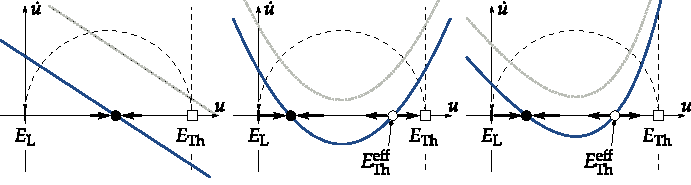
\includegraphics[trim=0cm 0cm 7.8cm 0cm,clip]{media/chp2/neuron_state_space.pdf}%
		\label{fig:lif_state}%
	}%
	\subbottom[QIF model]{%
		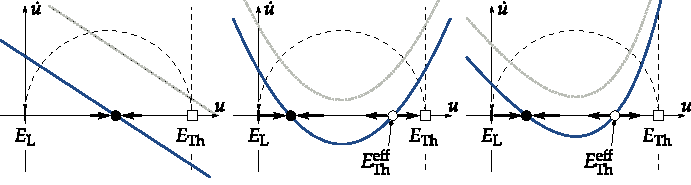
\includegraphics[trim=3.9cm 0cm 3.9cm 0cm,clip]{media/chp2/neuron_state_space.pdf}%
		\label{fig:qif_state}%
	}
	\subbottom[EIF model]{%
		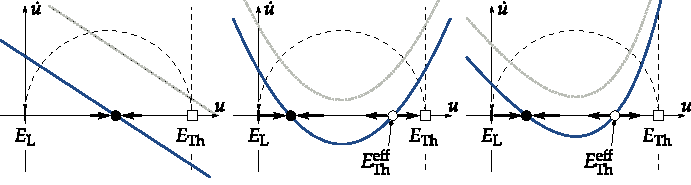
\includegraphics[trim=7.8cm 0cm 0cm 0cm,clip]{media/chp2/neuron_state_space.pdf}%
		\label{fig:eif_state}%
	}
	\caption[One dimensional integrate-and-fire model bifurcation patterns]{Sketch of one dimensional integrate-and-fire model bifurcation patterns. The three graphs show $\dum(\um)$ and the stationary points $\dum(\um) = 0$ for non-zero $\isyn$. Filled circles indicate stable stationary points, unfilled circles unstable stationary points. The reset mechanism is indicated by the unfilled box at $\um = \ETh$ and the dashed arrow pointing back at $\um$. The dotted grey lines show the same graph with a different choice for \isyn. Inspired by \cite{izhikevich2007dynamical}.}
	\label{fig:nlif_state}
\end{figure}

The \LIF neuron model has a severe instability in its dynamics: for $\El < \um < \ETh$, given $\isyn=0$, the differential $\dum(\um)$ in \cref{eqn:lif} evaluates to $\dum(\um) < 0$, even for infinitesimally small $\ETh - \um$. As shown in \cref{fig:lif_state}, it is only once \um reaches \ETh that an output \enquote{spike} is issued and the neuron is reset.

This behaviour has two major shortcomings. The model does not produce a sharp spike-formed action potential with a sudden rise in the membrane potential, and the biological phenomenon of \emph{spike latency} (\cref{fig:neuron_behaviours}(i), \cite{izhikevich2004model}) is not modelled: for a single short input current pulse the neuron might not spike immediately, but with a certain delay that decreases with the amplitude of the pulse.

\marginnote{The inner term in $f$ merely shifts and rescales the membrane potential \um, such that $\El$ maps to a dimensionless $0$ and $\ETh$ to $1$ (before $\El$ is subtracted).}
Spike generation and spike latency are modelled by non-linear integrate-and-fire neurons
\begin{align}
	- \Cm \cdot \dum(t) &= \Gl \cdot \left( f\left(\frac{\um(t) - 2 \cdot \El}{\ETh - \El}\right) \cdot (\ETh - \El) + \El \right) + \isyn
	\label{eqn:nlif} \,,
\end{align}
where $f$ is some non-linear function. If $f$ is chosen as the identity function, \cref{eqn:lif,eqn:nlif} are equivalent.

Examples for non-linear integrate-and-fire models are the \QIF and \EIF models: the corresponding functions $f$ with free parameters $f_1$, $f_2$ are given as
\begin{align}
	f_{\mathrm{QIF}}(u) &= - f_1 \cdot (u - f_2)^2
	& f_{\mathrm{EIF}}(u) &= u - f_1 \cdot \exp(u - f_2) \,.
	\label{eqn:nlif_f}
\end{align}
\marginnote{Care has to be taken when performing numerical integration of the equation, as the non-linearity might be numerically unstable.}
As shown in \cref{fig:qif_state,fig:eif_state} the behaviour of these two models is qualitatively equivalent: as soon as \um crosses a certain value \EThEff, the potential is quickly pushed towards \ETh. Analogously to the \LIF model, for $\um < \EThEff$ the membrane converges towards a stable stationary point. Location and existence of the two stationary points depends on the external input current \isyn.

\subsection{Two-dimensional Hodgkin-Huxley approximations: the AdEx model}
\label{sec:adex}

The above integrate-and-fire neuron models are one-\-dim\-en\-sio\-nal: their state vector solely consists of the membrane potential \um. As mentioned at the end of \cref{sec:lif}, one-dimensional models cannot account for many of the observed behavioural patterns in biological neurons, as the neuron state \um is reset along with each output spike. Surprisingly, most of the relevant behaviour of the \HH model (which has four state variables) can be modelled with only two-dimensions.

The Izhikevich model is a well-established and computationally cheap example of such an approximation \cite{izhikevich2004model}. Another interesting approximation is the \MAT model, which minimally extends the \LIF model with an adaptive threshold $\ETh(t)$. Due to its linearity, the model is numerically stable and yet very successful in approximating membrane potential traces recorded from biological neurons \cite{kobayashi2009made}.

\marginnote{The adaptation current $\iadap(t)$ can be biologically interpreted as a form of habituation or short-time plasticity \cite{kandel2012principles}.}
In this thesis we focus on the \AdEx model implemented in hardware in the \HBP physical model system \acrshort{NMPM}. Just as the above models, it is a two-dimensional non-linear integrate-and-fire model which reproduces a majority of the behavioural patterns observed in nature \cite{AdExp2005,AdExpScholarpedia2009}. In addition to the membrane potential $\um(t)$, the \AdEx model tracks an adaptation current $\iadap(t)$, which hyperpolarises the neuron. The current $\iadap(t)$ increases by a small constant $\ib$ with every generated output spike
\begin{align}
	\iadap(t) &\gets \iadap(t) + \ib \quad \text{on } \um(t) > \ETh \,.
	\label{eqn:adex_iadap}
\end{align}
\marginnote{The subthreshold adaptation allows to model the biological phenomenon of \enquote{threshold variability}, see \cref{fig:neuron_behaviours}(o).}
The adaptation current \iadap decays exponentially with a time constant \TauA and additionally depends on the \enquote{subthreshold adaptation conductance} $\Ga \geq 0$ which controls the influence of the membrane potential on the decay rate. For $\um(t) < \El$ the adaptation current decays faster, while $\um(t) > \El$ prolongs the decay:
\begin{align}
 	- \mathrm{d}/\mathrm{d}t \; \TauA \cdot \iadap(t) &= \iadap(t) - \Ga \cdot (\um(t) - \El) \,. \label{eqn:adex_tauA}
\end{align}

\marginnote{In the original \AdEx paper and corresponding code, \EThExp is usually referred to as \ETh, and \ETh is replaced by a potential \Espike.}
The model furthermore inherits the exponential spike generation mechanism from the \EIF model as described in \cref{eqn:nlif,eqn:nlif_f}. The final model equation is given as
\begin{align}
	\hspace{-0.2cm}-\Cm \cdot \dum(t) &= \Gl \cdot (\um(t) - \El) + \ITh(\um(t)) + \iadap(t) + \isyn(\um(t), t) \label{eqn:adex} \\
	\ITh(\um) &= \Gl \cdot \DT \cdot \exp \left(\frac{\um - \EThExp}{\DT}\right) \,.
	\label{eqn:adex_ith}
\end{align}
The exponential threshold potential \EThExp controls the minimum membrane potential $\um(t)$ at which the inner term of the exponential in $\ITh(u)$ is positive. For larger membrane potentials an exponentially rising current triggers an avalanche which causes the generation of an output spike. The parameter \DT controls the slope of the exponential current. While the rising spike onset is explicitly modelled, the falling edge is not. The same reset mechanism as in the \LIF model in \cref{eqn:lif_reset} is used, albeit the reset threshold \ETh is chosen considerably larger in the \AdEx model.


\begin{figure}
	\centering
	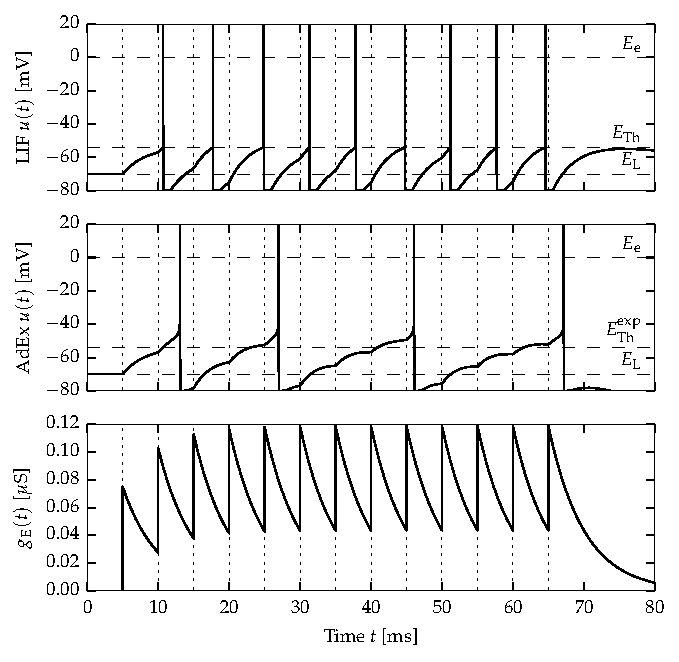
\includegraphics{media/chp2/lif_vs_adex.pdf}
	\caption[Comparison between the LIF and AdEx neuron models]{Comparison between the \LIF and \AdEx neuron models. The first two plots show the membrane potential of a \LIF and an \AdEx neuron, the bottom plot the conductance of a conductance based excitatory synapse, which receives 13 spikes in an interval of $\isi = \SI{5}{\milli\second}$. Due to the adaptation current, the output spike rate of the \AdEx neuron decreases over time, whereas the \LIF neuron outputs spikes at a constant rate. The spike potential at $\Espike = \SI{20}{\milli\volt}$ is artificially inserted by the simulator for the \LIF model, the \AdEx model intrinsically generates a spike onset.}
	\label{fig:lif_vs_adex}
\end{figure}

\cref{fig:lif_vs_adex} depicts a comparison of the behaviour of a \LIF and an \AdEx neuron with a conductance based synapse for a series of input spikes with equidistant timing. As a result of the adaptation current the output spike rate reduces over time.

\begin{table}
	\centering
	\small
	\newcommand{\SA}{\ensuremath{\circ}}
	\newcommand{\SB}{\ensuremath{\diamond}}
	\vspace*{0.45cm}
	\begin{tabular}{c l p{5.65cm} r r l}
		\toprule
		\multicolumn{6}{c}{\spacedlowsmallcaps{LIF and AdEx model parameters and typical values}} \\
		\midrule
		\multicolumn{6}{c}{\slshape Potentials} \\
		\midrule

			& & \spacedlowsmallcaps{Description} & \spacedlowsmallcaps{LIF} & \spacedlowsmallcaps{AdEx} & \\

			\noalign{\vskip 2mm}
			& \El  & Membrane leak or resting potential
			& $-65.0$ & $-70.6$ & [\si{\milli\volt}]\\

			\noalign{\vskip 2mm}
			& \ETh & Threshold potential. If passed, the neuron resets and issues an output spike.
 			& $-50.0$ & $-40.0$ & [\si{\milli\volt}] \\

			\noalign{\vskip 2mm}
			& \Ereset & Reset potential. Potential the membrane is reset to during the refractory period.
			& $-65.0$ & $-70.6$ & [\si{\milli\volt}] \\

			\noalign{\vskip 2mm}
		\SB & \Ee & Excitatory synapse reversal potential
			& $0.0$ & $0.0$ & [\si{\milli\volt}] \\

			\noalign{\vskip 2mm}
		\SB & \Ei & Inhibitory synapse reversal potential
			& $-70.0$ & $-80.0$ & [\si{\milli\volt}] \\

		\midrule
		\multicolumn{6}{c}{\slshape Time constants} \\
		\midrule

			& & \spacedlowsmallcaps{Description} & \spacedlowsmallcaps{LIF} & \spacedlowsmallcaps{AdEx} & \\

			\noalign{\vskip 2mm}
			& \TauRef & Duration of the refractory state
			& $0.1$ & $0.1$ & [\si{\milli\second}] \\

			\noalign{\vskip 2mm}
		\SB & \TauE & Excitatory synapse time constant
			& $5.0$ & $5.0$ & [\si{\milli\second}] \\

			\noalign{\vskip 2mm}
		\SB & \TauI & Inhibitory synapse time constant
			& $5.0$ & $5.0$ & [\si{\milli\second}] \\

		\midrule
		\multicolumn{6}{c}{\slshape Membrane parameters} \\
		\midrule

			& & \spacedlowsmallcaps{Description} & \spacedlowsmallcaps{LIF} & \spacedlowsmallcaps{AdEx} & \\

			\noalign{\vskip 2mm}
			& \Cm & Membrane capacitance
			& $1.0$ & $0.281$ & [\si{\nano\farad}] \\

			\noalign{\vskip 2mm}
			& \Gl & Membrane leak conductance
			& $0.05$ & $0.03$ & [\si{\micro\siemens}] \\

			\noalign{\vskip 2mm}
			& \TauM & Membrane time constant\newline ($\TauM = \Cm / \Gl$ )
			& $20.0$ & $9.37$ & [\si{\milli\second}] \\

		\midrule
		\multicolumn{6}{c}{\slshape AdEx adaptation and exponential current mechanism} \\
		\midrule

			& & \spacedlowsmallcaps{Description} & \spacedlowsmallcaps{LIF} & \spacedlowsmallcaps{AdEx} & \\

			\noalign{\vskip 2mm}
 		\SA & \Ga & Subthreshold adaptation
			& / & $4.0$ & [\si{\nano\siemens}] \\

			\noalign{\vskip 2mm}
		\SA & \ib & Spike-triggered adaptation current
			& / & $0.08$ & [\si{\nano\ampere}] \\

			\noalign{\vskip 2mm}
		\SA & \TauA & Adaptation current time constant
			& / & $144.0$ & [\si{\milli\second}] \\

			\noalign{\vskip 2mm}
		\SA & \EThExp & Exponential threshold potential
			& / & $-50.4$ & [\si{\milli\volt}] \\

			\noalign{\vskip 2mm}
		\SA & \DT & Exponential current slope
			& / & $2.0$ & [\si{\milli\volt}] \\

		\midrule
		\multicolumn{6}{c}{\slshape State variables} \\
		\midrule

			& & \spacedlowsmallcaps{Description} & \spacedlowsmallcaps{LIF} & \spacedlowsmallcaps{AdEx} & \\

			\noalign{\vskip 2mm}
			& $\um(t)$ & Membrane potential & / & / & [\si{\volt}] \\

			\noalign{\vskip 2mm}
		\SA & $\iadap(t)$ & Adaptation current & / & / & [\si{\ampere}] \\

			\noalign{\vskip 2mm}
		\SB & $\Ge(t)$ & Excitatory channel conductance & / & / & [\si{\siemens}] \\

			\noalign{\vskip 2mm}
		\SB & $\Gi(t)$ & Inhibitory channel conductance & / & / & [\si{\siemens}] \\
		\bottomrule
	\end{tabular}
	\caption[LIF and AdEx model parameters and state variables]{Parameters of the \LIF and \AdEx neuron models and state variables in conjunction with excitatory and inhibitory conductance based synapses. The typical values reflect the biologically motivated default parameters in \PyNN~0.8. \SA\ Only available in the AdExp model. \SB\ Synapse parameters.}
	\label{tbl:adex_parameters}
\end{table}
The \AdEx model can emulate the simpler \LIF model by setting the parameters \Ga and \ib to zero and deactivating the exponential threshold current \ITh, which -- depending on the implementation -- can be achieved by setting \DT to zero. \cref{tbl:adex_parameters} gives an overview of all parameters in the \AdEx and \LIF model with conductance based excitatory and inhibitory synapses.

\section{Neuromorphic hardware}
\label{sec:neuromorphic_hardware}

Biological spiking neural networks, including the human brain, are asynchronous, distributed, extremely parallel and stochastic. Classical digital computers on the other hand are synchronous, centralised, of limited parallelism and deterministic. They are conceivably ill-suited for time and energy efficient simulation of large-scale spiking neural networks. The term \emph{neuromorphic hardware} refers to systems which trade the versatility of general purpose computers with the architectural properties of central nervous systems and are specifically developed for a certain range of neural network models. Neural networks have been predominantly implemented in hardware in the 1950s and 1960s, when no powerful general purpose computers were available, see for example \cite{hay1960mark,widrow1960adaptive}. However, no system for brain-scale networks has been developed to date.

\marginnote{The description of the hardware systems in this chapter follows their specification, comments regarding the current state of the systems at the time of writing are given in \cref{chp:experiments}.}
Providing such neuromorphic hardware platforms is a central aim of the \HBP. Here, two complementary approaches are pursued. The physical model \acrshort{NMPM} simulates individual neurons and synapses as analogue physical model circuits. Conversely, the fully digital many-core system \acrshort{NMMC} consists of a vast number of conventional microprocessors, each of which simulates a small number of neurons. In both systems spikes are propagated over a digital, packet based, asynchronous and potentially unreliable communication network \cite{hbp_neuromorphic_platform}. In this section we describe \NMMC, \NMPM, its single-chip predecessor \enquote{Spikey} and the software stack provided to the end-user.

\subsection{NM-MC1: The many-core system}

The neuromorphic many-core system \NMMC is developed at the University of Manchester and based on the SpiNNaker chip, a multiprocessor designed for real-time simulation of spiking neural networks \cite{hbp_neuromorphic_platform}. Each chip contains up to 18 ARM968 processors running at a nominal frequency of $\SI{180}{\mega\hertz}$, with one processor dedicated to management purposes. Each processor has access to $32\,\mathrm{KiB}$ of instruction memory and $64\,\mathrm{KiB}$ data memory, while each chip connects to $128\,\mathrm{MiB}$ of external DDR SDRAM. Additionally, SpiNNaker features six bidirectional inter-chip communication links with integrated router used to exchange spike events over the network of chips during simulation. \NMMC consists of boards with 48 SpiNNaker chips each, organised in a torus network topology. \NMMC will eventually consist of ten cabinets with 120 boards each, resulting in a maximum of $979\,200$ processors for neural network simulation \cite{painkras2013spinnaker,furber2013overview}.

The system is theoretically capable of running any neuron model. However, the processors do not feature a floating-point unit, so in order to avoid the overhead of a software floating-point implementation, the neuron time dynamics are simulated with fixed-point arithmetic. As \mbox{\NMMC} is designed for the execution of spiking neural networks at biological timescale, the number of neurons per core varies with the computational complexity of the model. The system supports the \LIF model with both conductance and current based synapses, as well as the Izhikevich neuron model \cite{hbp_neuromorphic_platform, izhikevich2004model}. Algorithmically, the \LIF neuron dynamics are integrated using the Euler method at \SI{1}{\milli\second} timestep with 32-bit intermediate fixed-point values and 16-bit fixed-point parameter storage, allowing up to 256 \LIF neurons with conductance based synapses in a single core \cite{rast2010leaky}. Correspondingly, \NMMC can simulate up to 250 million neurons, which is two orders of magnitude smaller than the estimated number of neurons in the human cortex \cite{braitenberg2013cortex}.

\subsection{NM-PM1: The physical model}

\begin{figure}
	\centering
	\vspace*{0.4cm}
	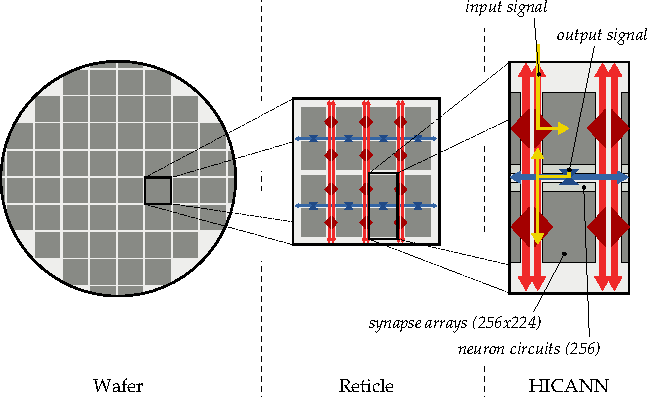
\includegraphics{media/chp2/nmpm1_sketch.pdf}\\
	\vspace*{0.4cm}
	\caption[NM-PM1 wafer high level architecture overview]{\NMPM wafer high level architecture overview. A single wafer in the NM-PM1 system consists of 384 \HICANN chips, organised in reticles. A \HICANN consists of two analogue blocks, each built of a synapse array and a neuron circuit. Each \HICANN is connected to an on-chip network, organised in horizontal buses (blue) receiving neuron output, and vertical buses (red) transmitting input signals to the synapse drivers. Adapted from \cite{petrovici2014characterization}.}
	\label{fig:nmpm1_sketch}
\end{figure}

\marginnote{Research on \HICANN and \NMPM originated in the European \FACETS and \BrainScaleS projects and is now continued in the \HBP.}
The neuromorphic physical model \NMPM is developed at the Kirchhoff Institute for Physics at Heidelberg University. \NMPM is built around the mixed-signal \HICANN (\acrlong{HICANN}) chip. Each \HICANN consists of two blocks, each hosting 256 analogue neuron circuits and a $224\times256$ matrix of analogue synapse circuits. Adjacent rows in the synapse matrix receive external input via synapse drivers (112 per block), which are connected to a digital on-chip communication network. To provide neurons with variable synapse count, up to 64 physical neuron circuits can be joined to form a logical neuron, allowing up to $14\,336$ synapses per logical neuron at the cost of reducing the number of logical neurons per block to a minimum of four. Each synapse can store a 4-bit weight. Synapse rows can be combined in order to achieve a higher weight resolution.

The analogue circuits on the chip emulate the dynamics of the \AdEx and \LIF models with excitatory and inhibitory conductance based synapses. Due to the analogue implementation it is important to distinguish model and hardware parameters: individual hardware parameters are mostly configured as voltages in analogue floating gates. The biological model parameters must be mapped onto these hardware parameters, taking calibration values for the individual circuits into account.
\marginnote{Alternatively, the speedup factor can specified by the user, but then only limited choices regarding the membrane capacitance \Cm are possible.}
As each neuron circuit can only be configured to use one of two membrane capacitances, the mapping process must not only adapt the model membrane potentials, currents, and conductivities to their hardware voltage representation, but also rescale the time constants to match the model membrane capacitance $\Cm$. This results in a speedup factor between $10^3$ and $10^5$ compared to biological timescale.

Apart from the $10^5$ speedup factor, another salient property of \NMPM is its wafer-scale integration: instead of separating the individual \HICANN chips from their silicon wafer after manufacturing, the wafer is left intact. Connections between the largest lithographic units -- the reticles -- are layered onto the wafer in a post-processing step. The wafer-scale approach is feasible, as errors in the analogue circuitry are tolerable (as they are in biological systems) and can be marked
\marginnote{While impressive, the number of neurons in \NMPM is still four magnitudes smaller than the estimated number of neurons in the human brain, but already close to the size of a mouse cortex \cite{braitenberg2013cortex}.}
as such in software. Each wafer comprises 384 {\HICANN}s, summing up to a theoretical maximum of $1\,966\,080$ neurons and $44$ million synapses \cite{petrovici2014characterization}. An overview of the organisational topology is depicted in \cref{fig:nmpm1_sketch}. In its final stage, \NMPM is planned to consist of 20 wafer systems, resulting in a total of $3.9$ million neurons \cite{hbp_neuromorphic_platform}. The \ESS allows to simulate parts of \NMPM without access to the actual hardware \cite{bruderle2011comprehensive}.

\subsection{Spikey}
\label{sec:spikey}

The Spikey analogue neuromorphic hardware system (\cref{fig:spikey}) has been developed as part of the \FACETS project at the University of Heidelberg. As a predecessor to \HICANN, the single Spikey chip in the system offers a speedup factor of $10\,000$ compared to biological timescale, and 384 analogue neurons, split into two blocks of 192 neurons each.
Each neuron implements a limited \LIF model and connects to 256 configurable analogue synapses with 4-bit weight resolution. Synapses are organised in 256 lines per block, with each line passing inputs from external or internal sources to the synapses. The neuron parameters \TauRef and \Gl can be chosen per neuron, all other neuron parameters are shared by groups of 96 neurons \cite{pfeil2013six}.

\subsection{Software stack}
\label{sec:pynn}

\begin{figure}
	\centering
	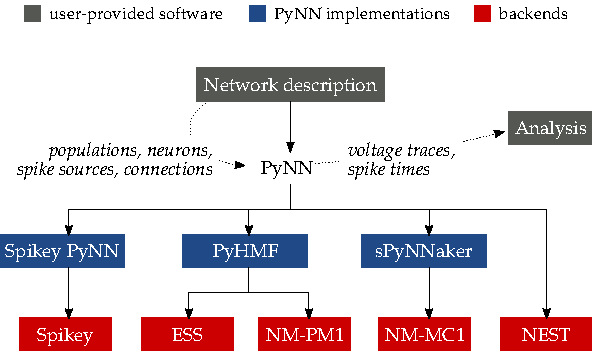
\includegraphics{media/chp2/pynn_software_stack.pdf}\\
	\caption[Neuromorphic hardware system software stack and data flow]{Neuromorphic hardware system software stack and data flow. Users provide a network description to \PyNN and request the recording of certain variables. Implementations of the \PyNN \acrshort{API} (blue) then communicate with the backend specific software (red). An interface for \NEST is directly included in \PyNN.}
	\label{fig:pynn_software_stack}
\end{figure}

Usually, neuromorphic hardware platforms, their emulators, and software simulators come with a native software interface specifically tailored to the system. For neuromorphic hardware, the backends map the network graph onto the neuromorphic substrate (place-and-route), convert the abstract neuron model parameters to concrete hardware parameters and perform the necessary communication tasks.

While the platform-provided libraries allow users to exploit specific platform features, their variety hinders the development of cross-platform network simulations, as each platform has to be targeted individually. To overcome this limitation, an \API with the name \PyNN is developed as part of \HBP \cite{davison2008pynn}. As shown in \cref{fig:pynn_software_stack}, \PyNN specifies a common software interface that allows to construct spiking neural network graphs, inject spike sources and flag neuron spike times and membrane potentials for recording. The individual developers of the hardware or software simulators provide an implementation of the \PyNN interface that communicates with the corresponding backend. This allows code written on top the \PyNN framework to run on arbitrary platforms, as long as it provides the required neuron models and the parameters are in the supported range.

Platforms targeted in this thesis via \PyNN are Spikey, \NMPM and its emulation \ESS, \NMMC and the software simulator \NEST. \NEST is developed at the Forschungszentrum Jülich as part of the research on large scale simulation of brain models on conventional high performance computing platforms in the \HBP \cite{gewaltig2007nest}. By design, \NEST is the most versatile and mathematically exact of the targeted platforms and acts as a reference system in this thesis.


%
% BINAM
%

\section{The Willshaw associative memory model (BiNAM)}
\label{sec:willshaw_theory}

\begin{figure}
	\footnotesize
	\centering
	\newlength{\tilewidth}
	\setlength{\tilewidth}{0.184\textwidth}
	\setlength{\tabcolsep}{2.75pt}
	\begin{tabular}{c c c c c}%
		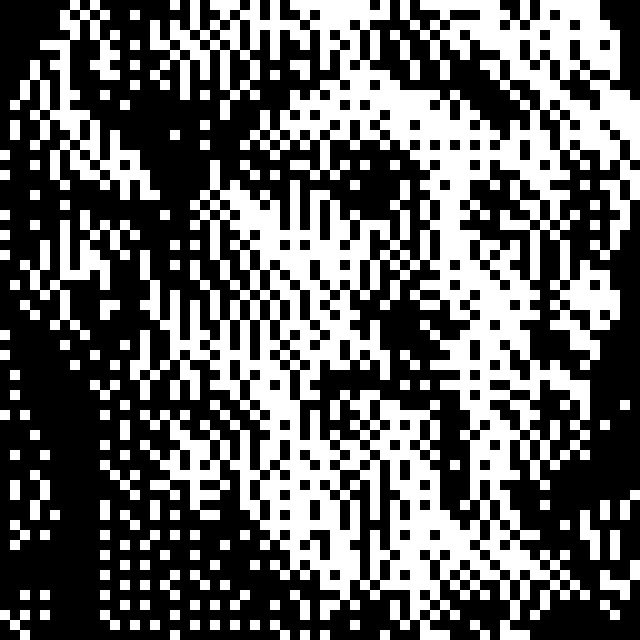
\includegraphics[width=\tilewidth,interpolate=false]{media/chp2/associative_memory/hopfield/04_00_orig_scaled_crushed.png}&%
		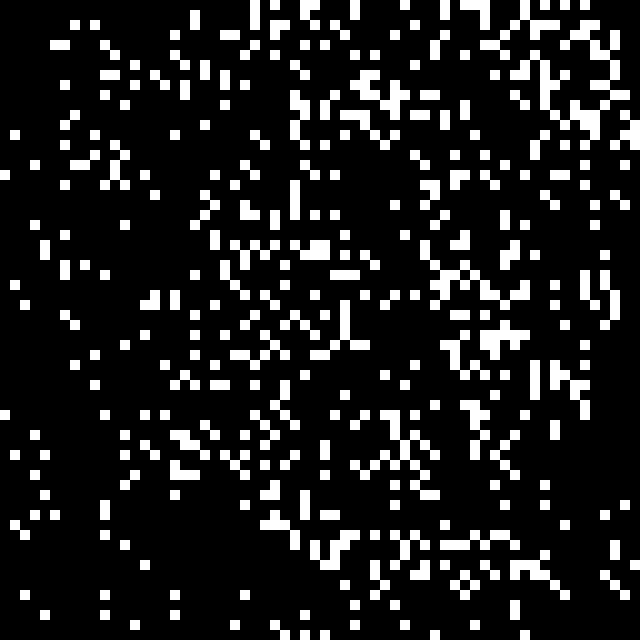
\includegraphics[width=\tilewidth,interpolate=false]{media/chp2/associative_memory/hopfield/04_01_noise_scaled_crushed.png}&%
		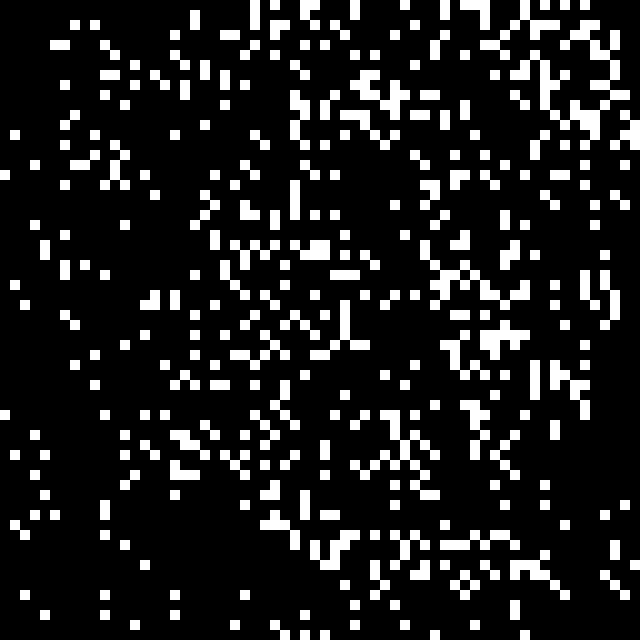
\includegraphics[width=\tilewidth,interpolate=false]{media/chp2/associative_memory/hopfield/04_02_activation_scaled_crushed.png}&%
		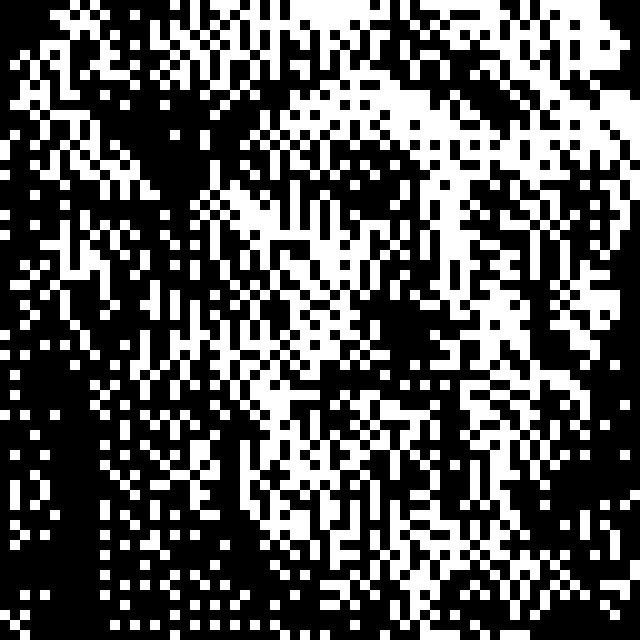
\includegraphics[width=\tilewidth,interpolate=false]{media/chp2/associative_memory/hopfield/04_03_activation_scaled_crushed.png}&%
		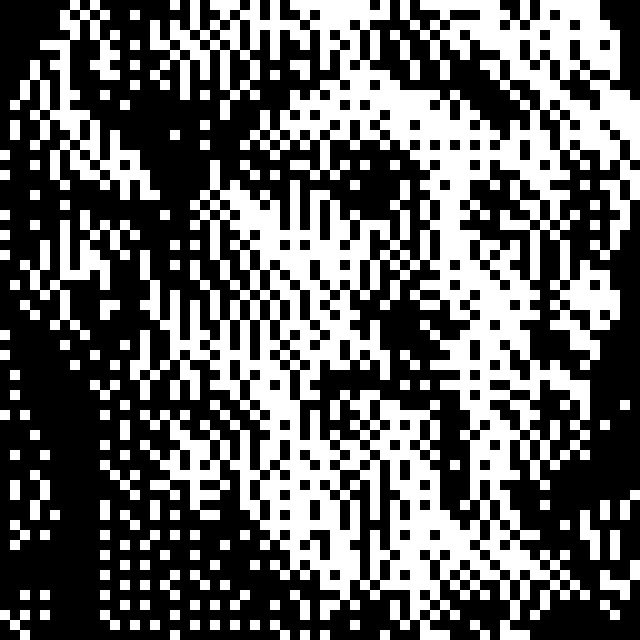
\includegraphics[width=\tilewidth,interpolate=false]{media/chp2/associative_memory/hopfield/04_04_activation_scaled_crushed.png}\\%
		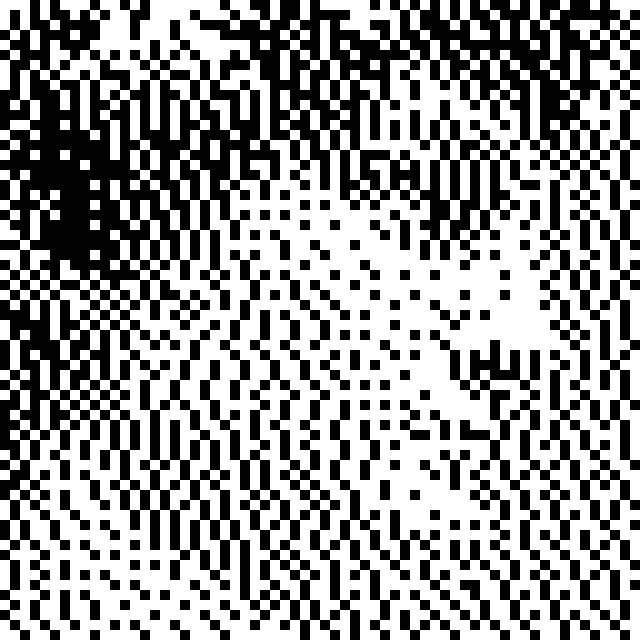
\includegraphics[width=\tilewidth,interpolate=false]{media/chp2/associative_memory/hopfield/05_00_orig_scaled_crushed.png}&%
		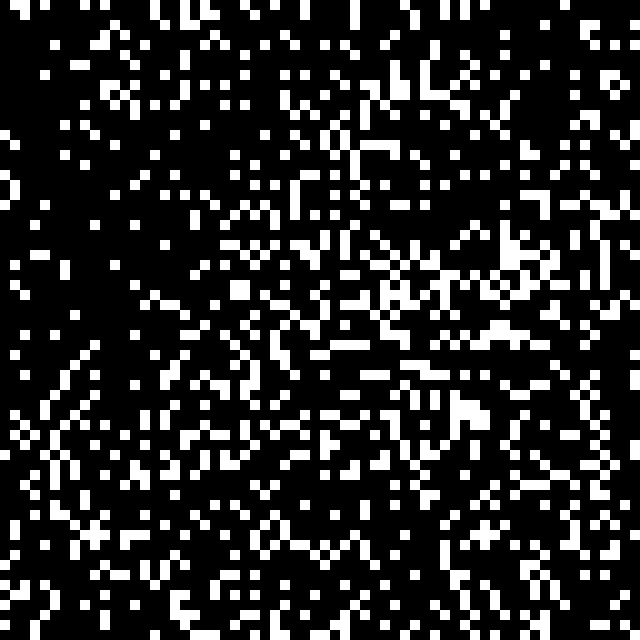
\includegraphics[width=\tilewidth,interpolate=false]{media/chp2/associative_memory/hopfield/05_01_noise_scaled_crushed.png}&%
		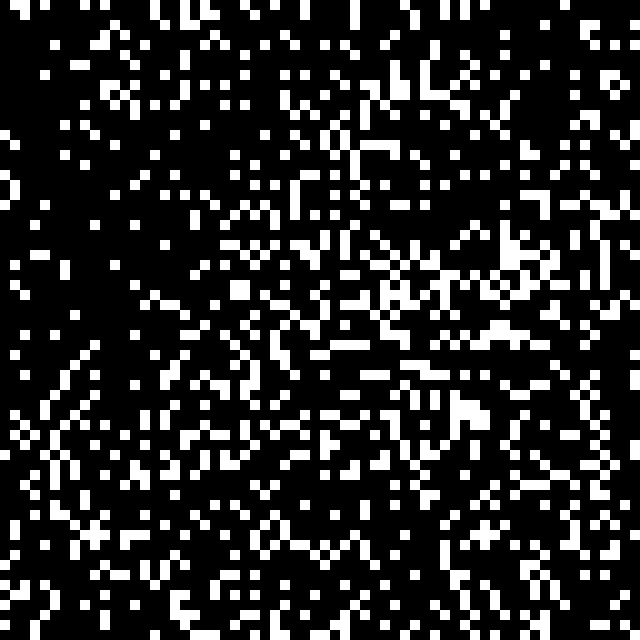
\includegraphics[width=\tilewidth,interpolate=false]{media/chp2/associative_memory/hopfield/05_02_activation_scaled_crushed.png}&%
		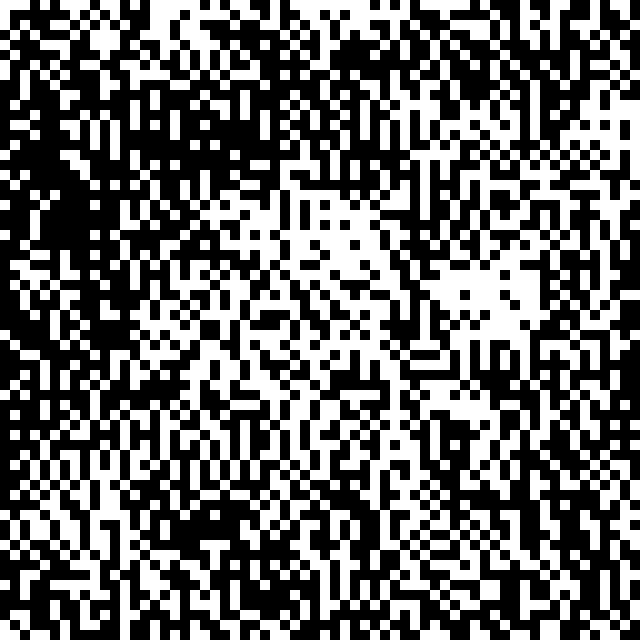
\includegraphics[width=\tilewidth,interpolate=false]{media/chp2/associative_memory/hopfield/05_03_activation_scaled_crushed.png}&%
		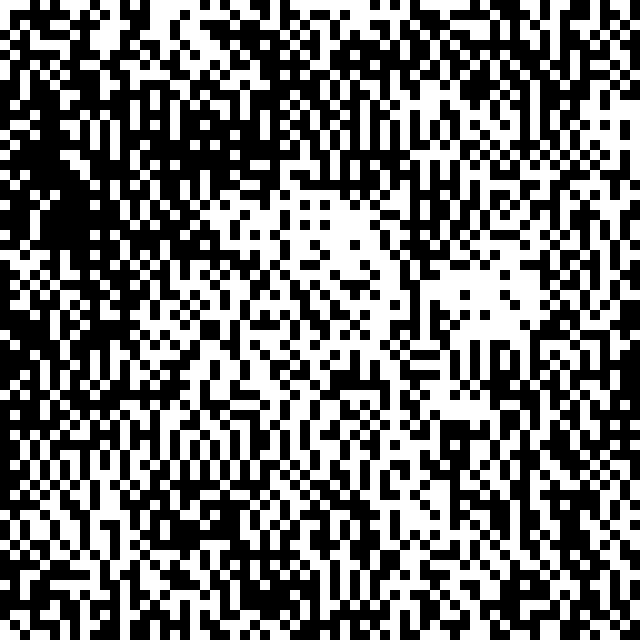
\includegraphics[width=\tilewidth,interpolate=false]{media/chp2/associative_memory/hopfield/05_04_activation_scaled_crushed.png}\\%
		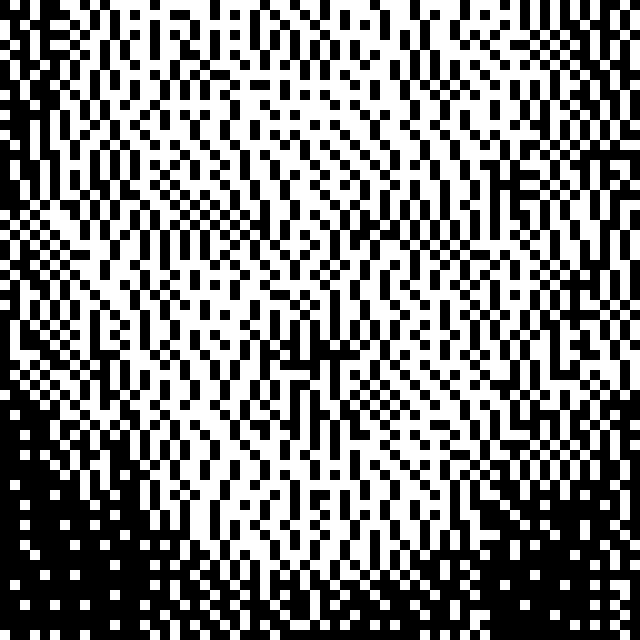
\includegraphics[width=\tilewidth,interpolate=false]{media/chp2/associative_memory/hopfield/06_00_orig_scaled_crushed.png}&%
		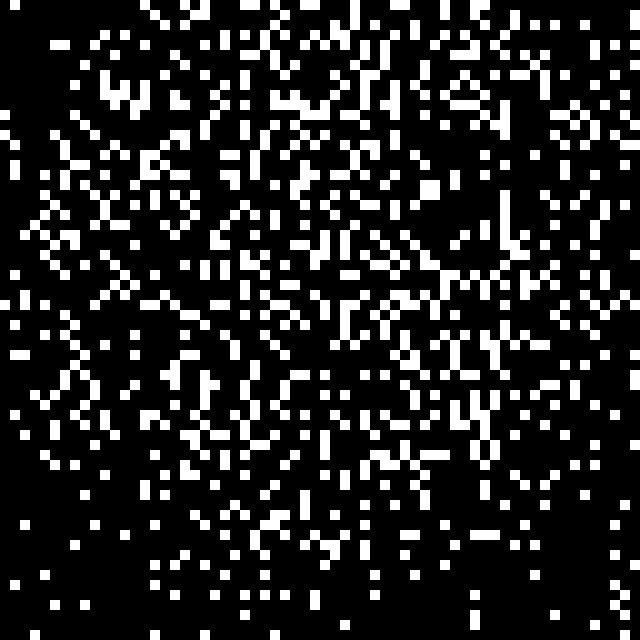
\includegraphics[width=\tilewidth,interpolate=false]{media/chp2/associative_memory/hopfield/06_01_noise_scaled_crushed.png}&%
		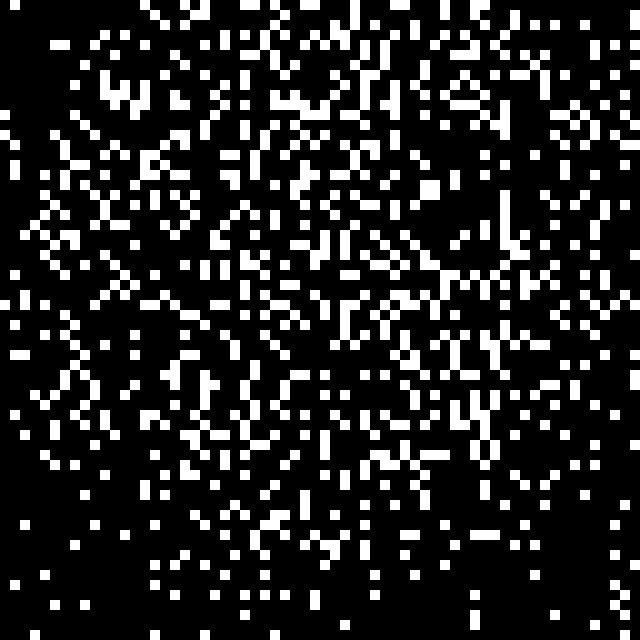
\includegraphics[width=\tilewidth,interpolate=false]{media/chp2/associative_memory/hopfield/06_02_activation_scaled_crushed.png}&%
		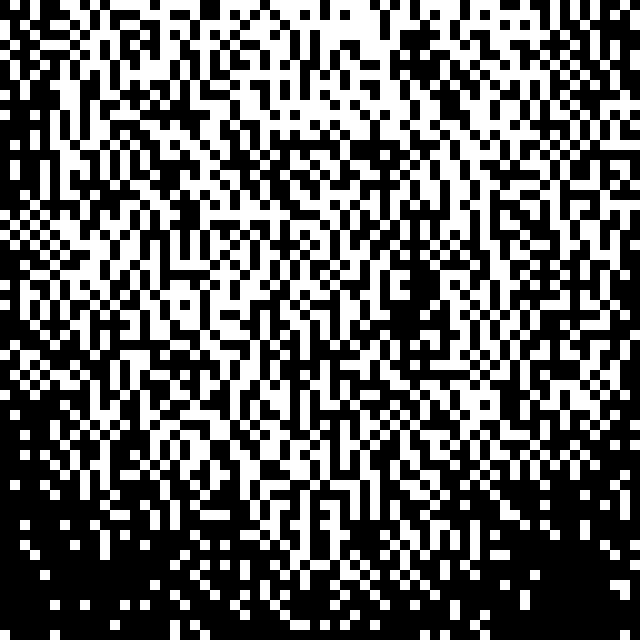
\includegraphics[width=\tilewidth,interpolate=false]{media/chp2/associative_memory/hopfield/06_03_activation_scaled_crushed.png}&%
		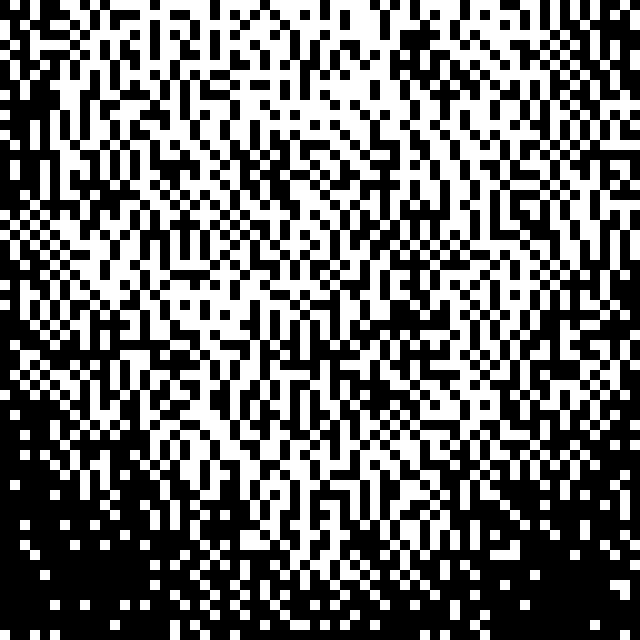
\includegraphics[width=\tilewidth,interpolate=false]{media/chp2/associative_memory/hopfield/06_04_activation_scaled_crushed.png}\\%
		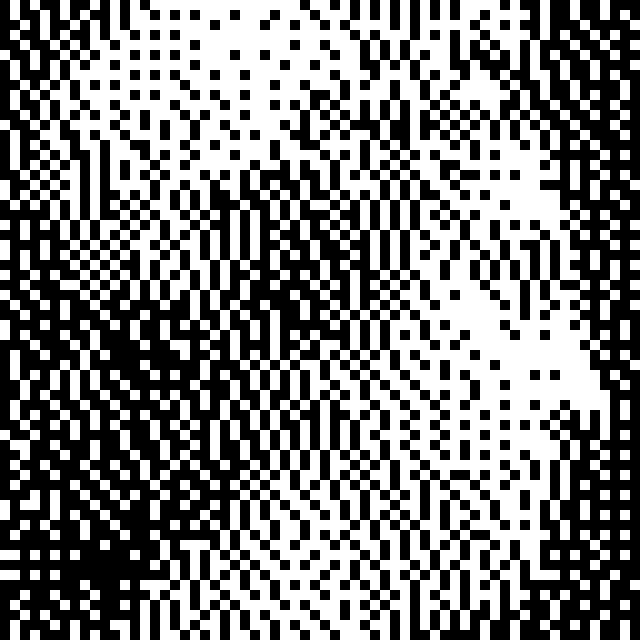
\includegraphics[width=\tilewidth,interpolate=false]{media/chp2/associative_memory/hopfield/07_00_orig_scaled_crushed.png}&%
		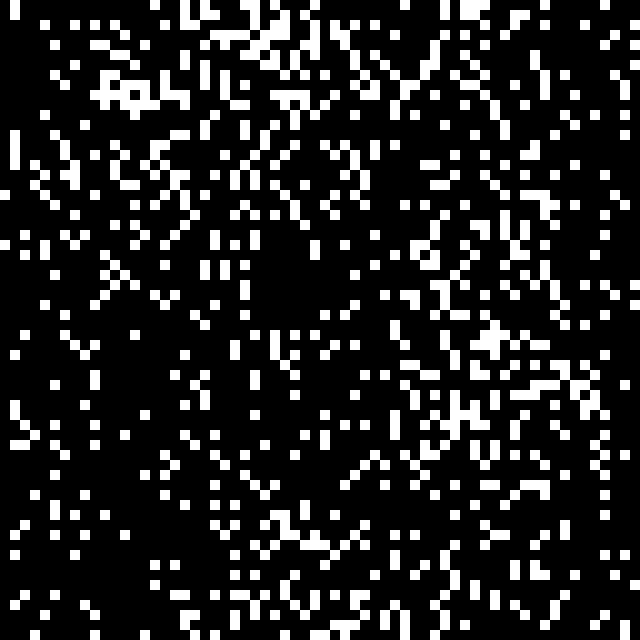
\includegraphics[width=\tilewidth,interpolate=false]{media/chp2/associative_memory/hopfield/07_01_noise_scaled_crushed.png}&%
		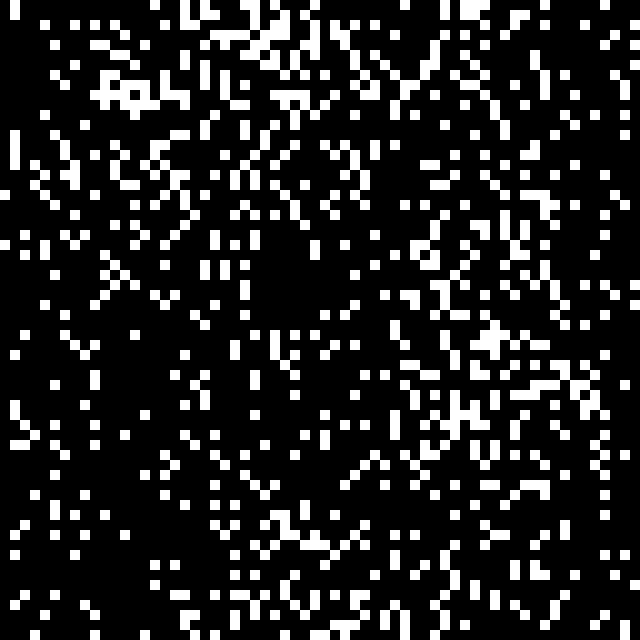
\includegraphics[width=\tilewidth,interpolate=false]{media/chp2/associative_memory/hopfield/07_02_activation_scaled_crushed.png}&%
		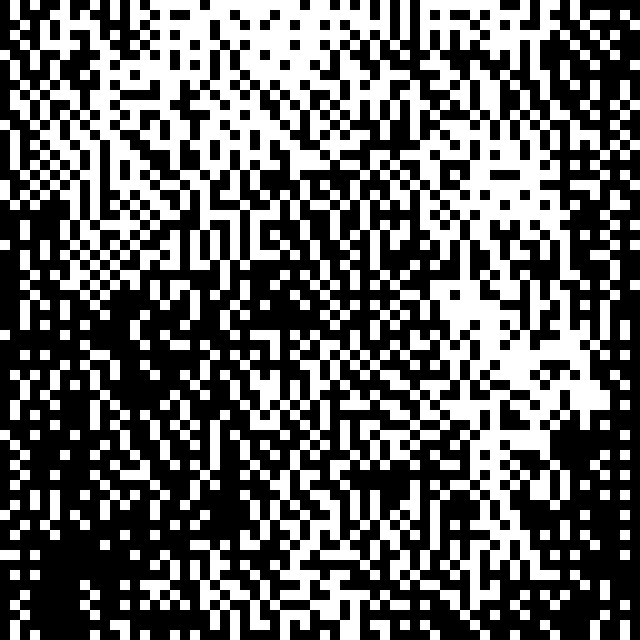
\includegraphics[width=\tilewidth,interpolate=false]{media/chp2/associative_memory/hopfield/07_03_activation_scaled_crushed.png}&%
		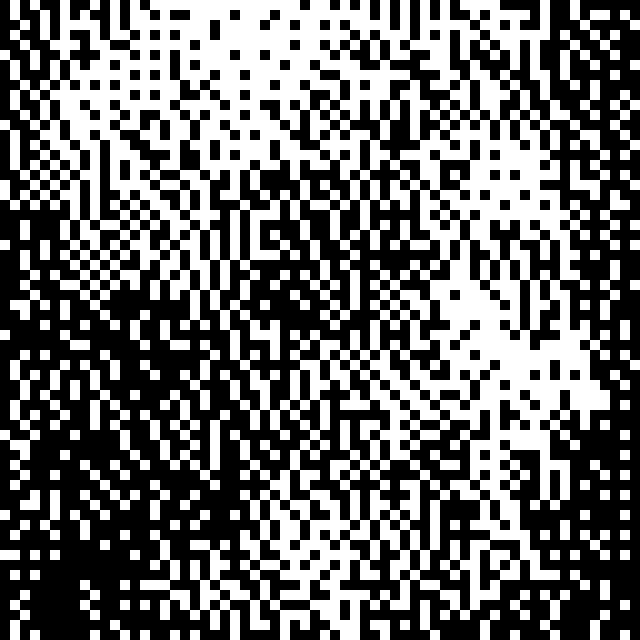
\includegraphics[width=\tilewidth,interpolate=false]{media/chp2/associative_memory/hopfield/07_04_activation_scaled_crushed.png}\\%
		(a) & (b) & (c) & (d) & (e)
	\end{tabular}
	\caption[Pattern completion in a Hopfield associative memory]{Example of pattern completion with a Hopfield associative memory. Column (a) shows $64 \times 64$ 1-bit images encoded as $4096$-dimensional column vectors $\vIn_k$. When presenting random $30\%$ of the original image as clue $\vIn$ to the memory (column (b)), it iteratively completes the patterns ((c)-(e)). Interference with four other stored images (not shown here) causes imperfect reproduction of the originals. The experiment is repeated with a \BiNAM in \cref{fig:binam_pattern_completion} (where all patterns are shown).}
	\label{fig:hopfield_pattern_completion}
\end{figure}

Along with artificial neural networks, technical implementations of associative memories have been researched since the middle of the last century, whereas the study of \enquote{associations} itself dates back to the ancient Greece philosopher Aristotle \cite{warren1916mental}. From our intuition it seems to be obvious that associations are an integral part of cognition: our brain constantly associates sensory input with internal states, such as feelings and memories, even if the two associated items are only connected remotely: consider the association of the smell of dry wood with the feeling of warmth at a fireplace. Of course, associations do not solely occur as a response to sensory input. Instead, they also play an important role in internal reasoning: often our mind follows a sequential chain of associations from one thought to the next until it suddenly \enquote{snaps} to the missing piece we have been searching for \cite{palm2013neural}.

Artificial associative memories aim at being high-level abstractions of the above concepts and merely touch the question on how associations actually work in human cognition. On the other hand, many associative memory models are implementable as neural networks and could be useful building blocks in artificial brain models. This section gives a quick conceptual overview of artificial associative memories and continues with a thorough description of the Willshaw model, its properties and implementation as a first-generation neural network.

\subsection{Artificial associative memory models}

Artificial associative memory models usually feature two phases: a \emph{training phase} in which input vectors $\vIn_k$ and the corresponding association $\vOut_k$ are presented to the model. In the \emph{recall phase} an arbitrary input vector $\vIn$ is fed into the system. In the optimal case the memory responds with the previously trained $\vOut_k$ corresponding to the trained input $\vIn_k$ to which $\vIn$ is closest according to a dissimilarity measure $\eth$
\begin{align}
	f(\vIn) = \vOut_k \quad \text{where} \quad k = \argmin_{k} \eth(\vIn_k, \vIn) \,.
	\label{eqn:associative_memory}
\end{align}
This concept resembles content addressed memory: data is not accessed by a physical address but by data itself, comparable to a hash map in computer science \cite{kohonen2012content}. Associative memories should also be clearly distinguished from function approximation in machine learning: the goal of associative memories is not to learn a generalised, continuous mapping between \vIn and \vOut, but to respond with one of the explicitly trained output vectors $\vOut_k$.

We distinguish two operational modes for associative memories: \emph{auto-association}, in which $\vIn_k = \vOut_k$ for all samples $k$, and \emph{hetero-association}, for which this equality is not presumed. As shown in \cref{fig:hopfield_pattern_completion}, auto-association can be interpreted as pattern-completion: given an altered (noisy) clue \vIn of a previously trained vector $\vIn_k$, the output of the memory converges towards a state resembling the original $\vIn_k$. Conversely, hetero-associations can be interpreted as semantic links between input $\vIn_k$ and output $\vOut_k$ \cite{palm2013neural}.

Hopfield networks, proposed in 1982, are one of the most famous associative memory models: they consist of a fully-connected network of McCulloch-Pitts cells (\cref{sec:mcculloch_pitts_neuron}) and operate on binary input and output vectors. During training, the synaptic weights $w_{ij}$ are set according to the \emph{Hebbian} learning rule \cite{hebb2005organization}. A connection between neuron $i$ and $j$ with $i \neq j$ is set to $w_{ij} = 1$ if $(\vIn_k)_i$ positively correlates with $(\vOut_k)_j$. Otherwise $w_{ij}$ is set to $w_{ij} = -1$
\begin{align}
	w_{ij} = \sign\left(\sum_{k} \big((\vIn_k)_i- \tfrac{1}2\big) \cdot \big( (\vOut_k)_j - \tfrac{1}2\big) \right) \,.
\end{align}
With this correlation based training scheme, the recurrent, fully-con\-nect\-ed network acts as a dynamical system with the trained output vector imprinted as attractors \cite{hopfield1982neural, hopfield2007hopfield}. Given an initial state $\vec x$, the network is likely to converge to the trained output $\vec y_k$ (\cref{fig:hopfield_pattern_completion}).

\subsection{Formal description of the Willshaw model}
\label{sec:binam_formal}

\marginnote{The output of the memory can of course be fed back to its input, which would result in a dynamical system and cause lots of fascinating behaviour. This is out of scope for this thesis.}
In contrast to Hopfield networks, the basic Willshaw associative memory model, or \acrfull{BiNAM}, does not describe a dynamical system. The model can be traced back to a paper by Steinbuch in 1961 \cite{steinbuch1961lernmatrix} and was independently described in 1969 by Willshaw \etal as a parallel, non-local and fault-tolerant associative network \cite{BiNAM1969}. It was further formalised and analysed by Palm \cite{palm1980associative}. Extensions of the model -- especially for spiking networks -- have, amongst others, been proposed by Knoblauch \cite{knoblauch2003synchronization, knoblauch2014structural}. Yet, as expounded in the introduction, we stick to the basic model.

Mathematically a \BiNAM can be defined as a binary storage matrix $\memMat \in \B^{\dimIn \times \dimOut}$, where $\B = \{0, 1\}$ is the base set of Boolean algebra, \dimIn is the dimensionality of the binary input vector $\vIn \in \B^{\dimIn}$ and \dimOut is the dimensionality of the output vector $\vOut \in \B^{\dimOut}$.

\paragraph{Training}
\begin{figure}
	\centering
	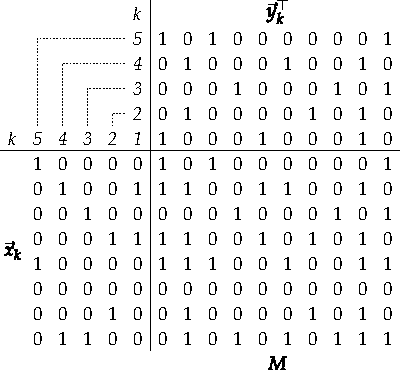
\includegraphics{media/chp2/binam_training.pdf}
	\caption[BiNAM training example]{Example of a $8 \times 10$ storage matrix \memMat after five samples $(\vIn_k, \vOut_k)$ with $\nOnesIn = 2$ ones in each input vector and $\nOnesOut = 3$ ones in each output vector have been trained according to \cref{eqn:binam_training}. The dotted lines connect input and output pairs.}
	\label{fig:binam_training}
\end{figure}
When training an association between an input $\vIn_k$ and output $\vOut_k$, the storage matrix \memMat is updated to a new \(\memMat'\)
\begin{align}
	\memMat' &= \memMat \vee \left( \vIn_k \cdot \transpose{\vOut_k} \right)\,,
	\label{eqn:binam_update_rule}
\end{align}
\marginnote{The condition \(\vIn_k = \vIn_\ell\) \(\Leftrightarrow k = \ell\) ensures unique input vectors: while it is possible for multiple \vIn to map to the same \vOut, it is prohibited for identical \vIn to map to multiple \vOut.}
where \enquote{$\vee$} is the element-wise \enquote{OR}-operation from standard Boolean algebra. If a set of \nSamples samples \((\vIn_k, \vOut_k)\)
\begin{align}
	\data = \{(\vIn_k, \vOut_k) \mid k \in \{1, \ldots, \nSamples\}\} \text{ with } \vIn_k = \vIn_\ell \Leftrightarrow k = \ell \,
	\label{eqn:binam_data}
\end{align}
is given in advance, a pre-calculated storage matrix \memMat can be obtained according to the following expression (\cref{fig:binam_training})
\begin{align}
	\memMat = \bigvee_{j = 1}^{\nSamples} \vIn_j \cdot \transpose{\vOut_j}\,.
	\label{eqn:binam_training}
\end{align}
\marginnote{Generation of data \data as used in the experiments conducted in this thesis is discussed in detail in \cref{sec:data_generation}.}
In this thesis we assume that such a pre-calculated storage matrix \memMat is already available --  we do not try to implement online training of the network. Additionally, and though not required for the operation of the \BiNAM, analysis of the memory is simplified significantly, if the number of bits set to \enquote{one} in both input and output vector is constant. We denote the number of \enquote{ones} in the input vectors \(\|\vIn_k\|_1\) as \(\nOnesIn\) and the number of \enquote{ones} in the output vectors \(\|\vOut_k\|_1\) as \(\nOnesOut\).

\paragraph{Recall}
\begin{figure}
	\centering
	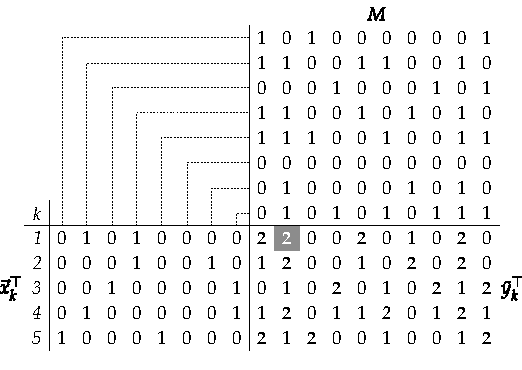
\includegraphics{media/chp2/binam_recall.pdf}
	\caption[BiNAM recall example]{Recalling the values associated to the \(\vIn_k\) previously trained in \cref{fig:binam_training}. The lower-right quadrant shows the intermediate results \(\transpose{\vOutI_k} = \transpose{\vIn_k} \cdot \memMat\) before applying the threshold function $\thresholdFunc_{\nOnesIn}$. Bold numbers correspond to those values that would be set to one in the final output, the grey backdrop signals a false-positive. The dotted lines connect rows in \memMat with their corresponding factors in the input data used when performing the vector-matrix multiplication.}
	\label{fig:binam_recall}
\end{figure}
In the recall phase, an arbitrary input vector \vIn is given. The output of the memory $\vOut$ can then be calculated as follows
\begin{align}
	\vOut &= \thresholdFunc_{\nOnesIn}(\vOutI) = 
		\thresholdFunc_{\nOnesIn}
			\left(\transpose{(\transpose{\vIn} \cdot \memMat)}\right)
		\quad \text{with} \quad
			\nOnesIn = \|\vIn\|_1 = \sum_{i = 0}^{\dimIn} (\vIn)_i = 
				\transpose{\vIn} \cdot \vIn\,,
	\label{eqn:binam_recall_rule}
\end{align}
\marginnote{Although the equation for \(\Theta_\theta\) looks fairly innocent, its realisation is the most crucial requirement for an operational spiking \BiNAM implementation.}
where $\thresholdFunc_{\threshold} : \N^{\dimIn} \longrightarrow \B^{\dimIn}$ is a step function with threshold \threshold, which maps the intermediate integer results of the matrix-vector multiplication \vOutI to binary values
\begin{align}
	(\thresholdFunc_{\threshold}(\vec z))_i
		&= \Heaviside\Big((\vec z)_i - \theta\Big) \,.
	\label{eqn:binam_threshold}
\end{align}
\cref{fig:binam_recall} shows the recall rule applied to the storage matrix \memMat previously trained in \cref{fig:binam_training}. As demonstrated, the recalled output of the \BiNAM is not perfect. A \emph{false positive} has been introduced (highlighted in grey): a one is present in component $j$ of the recalled output for \(\vIn_k\), although the trained \((\vOut_k)_j\) was set to zero.

\subsection{Choice of the threshold $\theta$}
\label{sec:binam_threshold}

Until now, the choice of \(\threshold = \nOnesIn\) in \cref{eqn:binam_recall_rule} has not been motivated. Consider a \BiNAM trained for a single sample \((\vIn_k, \vOut_k)\). The memory matrix is now set to $\memMat = \vIn_k \cdot \transpose{\vOut_k}$. Trying to recall \(\vOut_k\) by placing \(\vIn_k\) in \cref{eqn:binam_recall_rule} yields
\begin{align}
	\vOutI = \transpose{(\vIn_k \cdot \transpose{\vOut_k})} \cdot \vIn_k = \vOut_k \cdot (\transpose{\vIn_k} \cdot \vIn_k) = \vOut_k \cdot \nOnesIn \,.
\end{align}
Consequently, if a single sample is stored in the memory, the network returns an exact copy of the output vector \vOut scaled by \nOnesIn. Due to the additive superposition caused by the \enquote{$\vee$} in the training phase, newly trained samples can never lower the value of a single component $i$ in \vOutI, but only cause an increase towards the upper limit \nOnesIn
\begin{align}
%	\forall \memMat \in \B^{\dimIn \times \dimOut}, \vIn \in \B^{\dimIn}:
	(\vOutI)_i = (\transpose{\memMat} \cdot \vIn_k)_i \leq (\transpose{\memMat'} \cdot \vIn_k)_i \leq (\mathbb{1} \cdot \vIn_k)_i \leq \nOnesIn \,,
\end{align}
where $\mathbb{1}$ is the matrix of \enquote{ones} and
\begin{align}
	\memMat' &= \memMat \vee (\vIn \cdot \transpose{\vOut}) \text{ for any } \vIn \in \B^{\dimIn}, \vOut \in \B^{\dimOut}\,.
\end{align}
Given these considerations, adaptively setting the threshold \threshold to the maximum possible value $\nOnesIn = \|\vIn_k\|_1$, is the most sensible solution, as it minimises the chance of a false positive -- a bit in \vOut being set to one although it should be zero -- and yet prevents any \emph{false negatives}: all trained ones in the output are always present (see also \cref{sec:binam_failure_modes}).

\subsection{Storage capacity and sparsity}
\label{sec:binam_storage_capacity}

One of the defining properties of any memory is the amount of information that can be stored in the system. We refer to this measure as \emph{storage capacity}, or -- according to information theory -- \emph{information} or \emph{entropy}. Let us first consider the case of a conventional binary memory matrix \memMat of the size $\dimIn \times \dimOut$. Given a row index $k \in \{1, \ldots, \dimIn\}$ we can access any stored output vector $\vOut_k$. Each cell in $\vOut_k$ has two possible states, so the total number of possible $\vOut_k$ is $2^{\dimOut}$, and the number of possible matrices \memMat is $(2^{\dimOut})^{\dimIn}$. According to information theory, the number of bits \info needed to represent that many states is \cite{shannon2001mathematical}
\begin{align}
	\info = \lb((2^{\dimOut})^{\dimIn}) = \dimIn \cdot \lb(2^{\dimOut})= \dimIn \cdot \dimOut \,,
\end{align}
where $\lb$ is the binary logarithm. Given our constraint $\| \vOut_k \|_1 = \nOnesOut$, the amount of information is given as
\begin{align}
	\info = \lb\left(\binom{\dimOut}{\nOnesOut}^{\dimIn}\right) = \dimIn \cdot \lb \binom{\dimOut}{\nOnesOut}\,.
\end{align}

\begin{figure}[t]
	\centering
	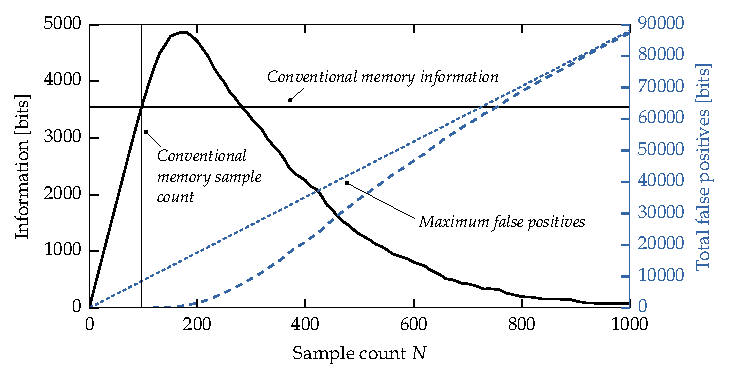
\includegraphics[trim=0.25cm 0.0cm 0.25cm 0.0cm,clip]{media/chp2/sketch_info.pdf}
	\caption[BiNAM information and false positive count over number of trained samples]{BiNAM information and false positive count over number of trained samples. Data size is $\dimIn = \dimOut = 96$, with $\nOnesIn = \nOnesOut = 8$. The optimal sample count is $\nSamples = 172$ with $\info = 4859$. For a conventional memory the same measures are $\nSamples = 96$ and $\info = 3\,547$.}
	\label{fig:sketch_info}
\end{figure}

\marginnote{For auto-associative storage measures see \cite{palm1980associative}.}
The same idea for the calculation of \info can be applied to associative memories in the hetero-association mode \cite{palm1980associative}. The only important difference between conventional and associative memories is the indexing scheme: output vectors $\vOut_k$ are not accessed by a row index $k$ but by a unique vector $\vIn_k$. In the case that all $\nSamples$ trained samples can be recalled perfectly, the storage capacity would be:
\begin{align}
	\info = \nSamples \cdot \lb \binom{\dimOut}{\nOnesOut}
\end{align}
\marginnote{The binomial coefficient $$\binom{\nOnesOut + \nFPk}{\nOnesOut}$$ expresses the number of ways in which the correct \nOnesOut ones can be distributed amongst the total number of ones in the output.}
However, as explained in \cref{sec:binam_threshold}, the probability of false positive bits in the output increases with the number of trained samples. Given the number of false positives \nFPk for a specific sample $k$, the possible number of states occupied by those wrong bits needs to be subtracted in the information calculation:
\begin{align}
	\info = \sum_{k = 1}^{\nSamples} \lb \binom{\dimOut}{\nOnesOut} - \lb \binom{\nOnesOut + \nFPk}{\nOnesOut}
	\label{eqn:binam_entropy}
\end{align}
If \nFNk false negatives are present in the output for sample $k$ (\cref{sec:binam_failure_modes}), an adapted equation must be used \cite{ruckert1991tolerance}:
\begin{align}
	\info = \sum_{k = 1}^{\nSamples}
			\lb\binom{\dimOut}{\nOnesOut}
		  - \lb\binom{\nFPk + \nOnesOut - \nFNk}{\nOnesOut - \nFNk}
		  - \lb\binom{\dimOut - \nFPk - \nOnesOut + \nFNk}{\nFNk}
	\label{eqn:binam_entropy_false_negatives}
\end{align}
As false positive and negative counts \nFPk and \nFNk are specific to the stored dataset and the actual $\vIn$ used for the recall operations, the storage capacity depends -- in contrast to conventional memory -- on memory content. \cref{fig:sketch_info} shows a simple experiment: a \BiNAM is trained with random data one sample at a time. After each sample has been trained, the stored information is calculated according to \cref{eqn:binam_entropy}, resulting in a characteristic information over sample count curve:
\marginnote{Achieving a higher storage capacity than conventional memories can be interpreted as intrinsic data compression in the \BiNAM. Given the information in the input $\vIn$, the $\vOut_k$ can be decompressed.}
the storage capacity \info quickly increases with the number of stored samples $\nSamples$, up to a certain maximum, and then converges to $\info = 0$ for large sample counts. In this particular example both the storage capacity \info and the number of stored samples significantly outperform the conventional memory.

However, this comes at a cost: for once, there is a chance of false positives in the output (the memory is not perfect) and the high storage capacity can only be reached if input and output vectors are \emph{sparse}: optimal performance is achieved if the number of ones $\nOnesIn, \nOnesOut$ are chosen logarithmic with respect to $\dimIn, \dimOut$. For non-sparse data the memory matrix \memMat converges to $\mathbb{1}$ too quickly, causing an increased false positive count \nFPk.

Note that the above restriction does not imply that the \BiNAM will not operate properly for non-sparse data -- the maximum storage capacity and the corresponding optimal sample count will just be smaller than that of conventional memories of the same size. An example of dense data storage in a \BiNAM is shown in \cref{fig:binam_pattern_completion}, which repeats the introductory pattern completion experiment from the beginning of this chapter with a \BiNAM instead of a Hopfield network. In contrast to the Hopfield network, the \BiNAM recalls all stored images perfectly in a single step.

Another conceptual property of the \BiNAM model is that it can be interpreted as a generalisation of a conventional memory. It gracefully reduces to such a memory if the $\vIn$  are appointed to \enquote{column selectors} which contain a single \enquote{one}, corresponding to $c = \|\vIn\| = 1$. Let, without any loss of generality, assume that the $\vIn_k$ are sorted such that $(\vIn_k)_k = 1$ and $\nSamples = \dimIn$
\begin{align}
	\memMat = \bigvee_{k = 1}^{\dimIn} \vIn_k \cdot \transpose{\vOut_k} = \transpose{(\vOut_1, \ldots \vOut_{\dimIn})} \Rightarrow \transpose{M} \cdot \vIn_k = \vOut_k \,.
\end{align}

\begin{figure}
	\footnotesize
	\centering
	\setlength{\tilewidth}{0.15\textwidth}
	\setlength{\tabcolsep}{2.75pt}
	\begin{tabular}{c c c c c c}%
		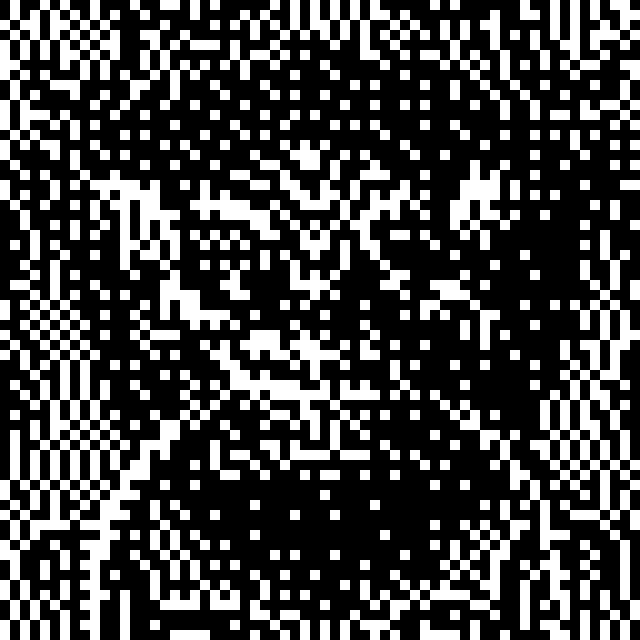
\includegraphics[width=\tilewidth,interpolate=false]{media/chp2/associative_memory/binam/00_00_orig_scaled_crushed.png}&%
		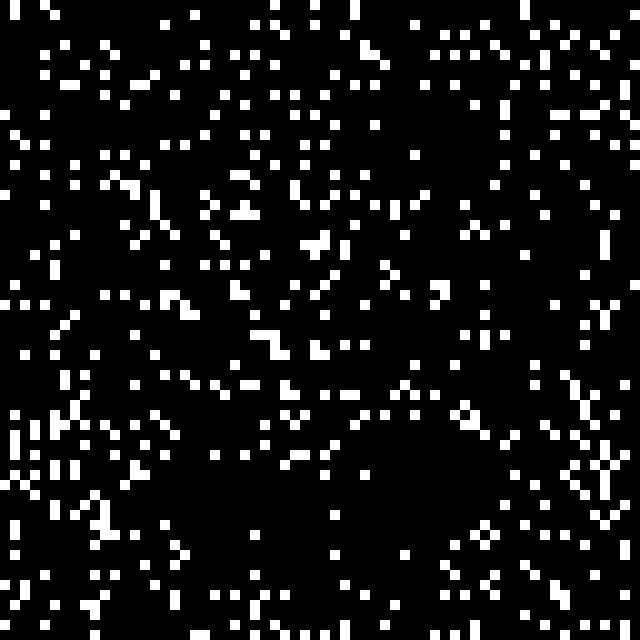
\includegraphics[width=\tilewidth,interpolate=false]{media/chp2/associative_memory/binam/00_01_noise_scaled_crushed.png}&%
		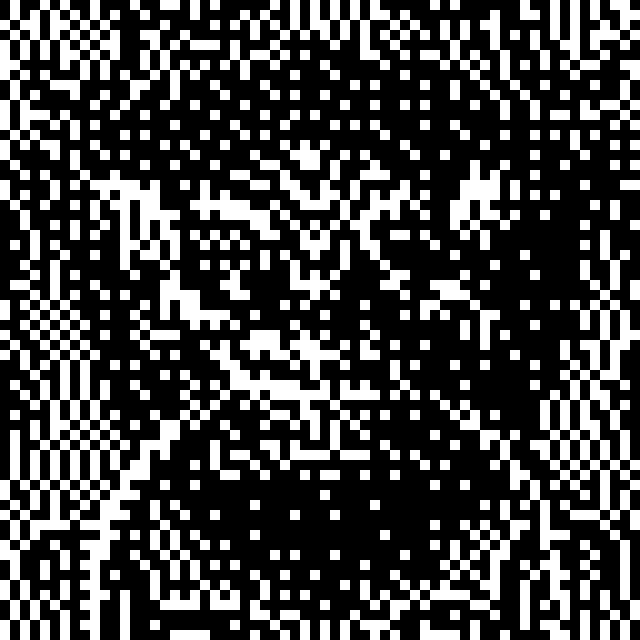
\includegraphics[width=\tilewidth,interpolate=false]{media/chp2/associative_memory/binam/00_02_out_scaled_crushed.png}&%
		
\includegraphics[width=\tilewidth,interpolate=false]{media/chp2/associative_memory/binam/01_00_orig_scaled_crushed.png}&%
		\includegraphics[width=\tilewidth,interpolate=false]{media/chp2/associative_memory/binam/01_01_noise_scaled_crushed.png}&%
		\includegraphics[width=\tilewidth,interpolate=false]{media/chp2/associative_memory/binam/01_02_out_scaled_crushed.png}\\
		\includegraphics[width=\tilewidth,interpolate=false]{media/chp2/associative_memory/binam/02_00_orig_scaled_crushed.png}&%
		\includegraphics[width=\tilewidth,interpolate=false]{media/chp2/associative_memory/binam/02_01_noise_scaled_crushed.png}&%
		\includegraphics[width=\tilewidth,interpolate=false]{media/chp2/associative_memory/binam/02_02_out_scaled_crushed.png}&%
		\includegraphics[width=\tilewidth,interpolate=false]{media/chp2/associative_memory/binam/03_00_orig_scaled_crushed.png}&%
		\includegraphics[width=\tilewidth,interpolate=false]{media/chp2/associative_memory/binam/03_01_noise_scaled_crushed.png}&%
		\includegraphics[width=\tilewidth,interpolate=false]{media/chp2/associative_memory/binam/03_02_out_scaled_crushed.png}\\
		\includegraphics[width=\tilewidth,interpolate=false]{media/chp2/associative_memory/binam/04_00_orig_scaled_crushed.png}&%
		\includegraphics[width=\tilewidth,interpolate=false]{media/chp2/associative_memory/binam/04_01_noise_scaled_crushed.png}&%
		\includegraphics[width=\tilewidth,interpolate=false]{media/chp2/associative_memory/binam/04_02_out_scaled_crushed.png}&%
		\includegraphics[width=\tilewidth,interpolate=false]{media/chp2/associative_memory/binam/05_00_orig_scaled_crushed.png}&%
		\includegraphics[width=\tilewidth,interpolate=false]{media/chp2/associative_memory/binam/05_01_noise_scaled_crushed.png}&%
		\includegraphics[width=\tilewidth,interpolate=false]{media/chp2/associative_memory/binam/05_02_out_scaled_crushed.png}\\
		\includegraphics[width=\tilewidth,interpolate=false]{media/chp2/associative_memory/binam/06_00_orig_scaled_crushed.png}&%
		\includegraphics[width=\tilewidth,interpolate=false]{media/chp2/associative_memory/binam/06_01_noise_scaled_crushed.png}&%
		\includegraphics[width=\tilewidth,interpolate=false]{media/chp2/associative_memory/binam/06_02_out_scaled_crushed.png}&%
		\includegraphics[width=\tilewidth,interpolate=false]{media/chp2/associative_memory/binam/07_00_orig_scaled_crushed.png}&%
		\includegraphics[width=\tilewidth,interpolate=false]{media/chp2/associative_memory/binam/07_01_noise_scaled_crushed.png}&%
		\includegraphics[width=\tilewidth,interpolate=false]{media/chp2/associative_memory/binam/07_02_out_scaled_crushed.png}\\
		(a) & (b) & (c) & (a) & (b) & (c)
	\end{tabular}
	\caption[BiNAM pattern completion experiment]{BiNAM pattern completion experiment with non-sparse vectors: the binary $64 \times 64$ pixel images in the (a) columns are trained as 4096-dimensional vectors $\vIn_k$. Random $30\%$ of the \enquote{ones} in the original image are then presented as clue $\vIn$ to the memory (b). The recalled result is shown in (c). In this example all images are perfectly recalled by the \BiNAM.}
	\label{fig:binam_pattern_completion}
\end{figure}

\subsection{Neural network implementation}
\label{sec:binam_neural_network}

\begin{figure}
	\centering
	\includegraphics{media/chp2/binam_network.pdf}\\
	\caption[Neural network implementation of the BiNAM]{Neural network implementation of the BiNAM with McCulloch-Pitts cells. The $x_1, \ldots, x_{\dimIn}$ correspond to the components of an input vector $\vIn$, the $y_1, \ldots, y_{\dimOut}$ to the components of the output vector $\vOut$. Dots in the intersections between the neural input and the input components correspond to an excitatory synapse. These are inserted for all $i, j$ with $(\memMat)_{i, j} = 1$. The threshold \threshold is fixed in this implementation.}
	\label{fig:binam_network}
\end{figure}

Since its inception, the \BiNAM model has been proposed as \enquote{biologically plausible}: it can be easily implemented as a first- or second-generation artificial neural network, and the corresponding topology resembles certain structures in the brain \cite{BiNAM1969, palm1980associative}. Yet, before we consider the implementation, two notes should be taken into account: as already mentioned, our implementation is not capable of online training. Furthermore, it does not provide dynamic threshold adaptation. The impact of a fixed threshold \threshold is discussed in \cref{sec:binam_failure_modes}.

\marginnote{Of course, the model can also be implemented as firing-rate network: in this case, the threshold function $\thresholdFunc_{\threshold}$ has to be used as non-linearity $f$.}
Due to its binary nature, the \BiNAM model can be perfectly implemented with the McCulloch-Pitts neuron model (\cref{sec:mcculloch_pitts_neuron}). The network as shown in \cref{fig:binam_network} consists of a single layer of \dimOut neurons which receive the input signal \vIn, either as external input or from a sub-network. Each neuron corresponds to a single output component in \vOut. An excitatory synapse is added between input component $i$ and output neuron $j$ if, and only if, $(\memMat)_{i, j} = 1$. The threshold \threshold should be set to the average number of \enquote{ones} \nOnesIn in the trained input. Smaller or larger values than \nOnesIn may be required if noise is present in \vIn.

\subsection{Impact of noise}
\label{sec:binam_failure_modes}

% \info und I verwechslung

\begin{figure}[t]
	\centering
	\includegraphics{media/chp2/sketch_info_over_noise.pdf}\\
	\vspace*{0.25cm}
	\includegraphics{media/chp2/sketch_fps_over_noise.pdf}
	\includegraphics{media/chp2/sketch_fns_over_noise.pdf}
	\caption[Information measure and error count over noise]{Information measure and error count over noise parameters \pFn and \pFp. A \BiNAM of size $\dimIn = \dimOut = 96$ is trained with  $\nSamples = 172$ samples with $\nOnesIn = \nOnesOut = 8$ one-bits. The graphs show the total information and the averaged false positive and false negative counts for the recall of all trained samples. Addition and omission of bits are performed with probabilities \pFn and \pFp. The behaviour between fixed and adaptive threshold \threshold is compared. In the fixed threshold case $\threshold = \dimIn = 8$.}
	\label{fig:sketch_info_over_noise}
\end{figure}

Aside from the pattern completion example in \cref{fig:binam_pattern_completion}, perfect conditions were assumed up to this point: the input vectors $\vIn_k$ presented to the network in the recall phase are the same as in the input data \data actually learned in the training phase. As noted above, even in this scenario there is the possibility of \emph{false positives}. This failure mode results from the storage matrix continuously getting saturated during training. If the \enquote{ones} in the training samples are uniformly distributed, the memory matrix \memMat asymptotically approaches the \enquote{ones} matrix $\mathbb{1}$ (\cref{sec:binam_random_data_behaviour}).

There are two ways in which we can corrupt the originally trained input vectors $\vIn_k$: by addition (additional bits are set to one) and by omission (bits originally set to one are set to zero). In the case of additive noise, the input vector \vIn can be modelled as
\begin{align}
	(\vIn)_i = (\vIn_k)_i \vee \eta \text{ with } \probability{(\eta = 0)} = 1 - \pFp \text{ and } \probability{(\eta = 1)} = \pFp \,,
\end{align}
where \pFp is the probability of an arbitrary input vector component being set to one. In the omission (multiplicative) case, the input vector \vIn can be modelled as
\begin{align}
	(\vIn)_i = (\vIn_k)_i \wedge \eta \text{ with } \probability{(\eta = 0)} = \pFn \text{ and } \probability{(\eta = 1)} = 1 - \pFn \,,
\end{align}
where \pFn is the probability of an arbitrary input vector component being set to zero. 

\cref{fig:sketch_info_over_noise} shows the impact of the two kinds of noise on storage capacity, \emph{false positive} and \emph{false negative} counts. It furthermore distinguishes between an adaptive threshold $\threshold = \|\vIn\|_1$ and a fixed threshold $\threshold$. For multiplicative noise and adaptive threshold, the information \info decreases almost linearly with \pFn. Counter-intuitively, the false-positive count increases the more bits are omitted in the input. This is caused by the missing input bits lowering the threshold \threshold. For a fixed threshold, the false-positive count converges to zero with increasing \pFn, accompanied with an increase in the false-negative count. Correspondingly, the information measure drops to zero.

Additive noise has a much stronger negative impact on the storage capacity as its multiplicative counterpart. First of all, this is caused by \pFp and \pFn not being directly comparable: due to sparsity, the probability of adding an additional \enquote{one} to the input is higher than setting an actual \enquote{one} to zero in the multiplicative case. If no adaptive threshold is used, the false positive count quickly rises towards the maximum. With adaptive threshold, the addition of input bits causes false negatives as the increased threshold masks the correct \enquote{ones}. In both cases the information measure \info drops to zero.

To summarise the possible \BiNAM failure modes: false positives can always be produced, even without noise. False negatives occur if input bits are missing and the threshold is not adapted (as in our neural network implementation, \cref{sec:binam_neural_network}), and if \threshold is increased above \nOnesIn due to additional input bits.


\section{Summary and outlook}

This chapter provided a scenic overview of various fields of research. We discussed neural network models, both from the view of neurobiology and neuroinformatics, and their implementation in neuromorphic hardware. Furthermore, we have thoroughly investigated the Willshaw associative memory and provided an implementation in the form of an artificial, first-generation neural network.

In \cref{chp:spinam}, we combine these building-blocks: we extend our \BiNAM implementation towards spiking neural networks and provide the workflow for design space exploration. In \cref{chp:neuron_evaluation}, we dive back into the details of the \LIF and \AdEx spiking neural network models to find proper values for the neuron parameters listed in \cref{tbl:adex_parameters}. Finally, in \cref{chp:experiments}, we pioneer into the realm of neuromorphic hardware and boldly execute the model on platforms, on which no associative memory has run before.
